% Options for packages loaded elsewhere
\PassOptionsToPackage{unicode}{hyperref}
\PassOptionsToPackage{hyphens}{url}
%
\documentclass[
]{article}
\usepackage{amsmath,amssymb}
\usepackage{lmodern}
\usepackage{ifxetex,ifluatex}
\ifnum 0\ifxetex 1\fi\ifluatex 1\fi=0 % if pdftex
  \usepackage[T1]{fontenc}
  \usepackage[utf8]{inputenc}
  \usepackage{textcomp} % provide euro and other symbols
\else % if luatex or xetex
  \usepackage{unicode-math}
  \defaultfontfeatures{Scale=MatchLowercase}
  \defaultfontfeatures[\rmfamily]{Ligatures=TeX,Scale=1}
\fi
% Use upquote if available, for straight quotes in verbatim environments
\IfFileExists{upquote.sty}{\usepackage{upquote}}{}
\IfFileExists{microtype.sty}{% use microtype if available
  \usepackage[]{microtype}
  \UseMicrotypeSet[protrusion]{basicmath} % disable protrusion for tt fonts
}{}
\makeatletter
\@ifundefined{KOMAClassName}{% if non-KOMA class
  \IfFileExists{parskip.sty}{%
    \usepackage{parskip}
  }{% else
    \setlength{\parindent}{0pt}
    \setlength{\parskip}{6pt plus 2pt minus 1pt}}
}{% if KOMA class
  \KOMAoptions{parskip=half}}
\makeatother
\usepackage{xcolor}
\IfFileExists{xurl.sty}{\usepackage{xurl}}{} % add URL line breaks if available
\IfFileExists{bookmark.sty}{\usepackage{bookmark}}{\usepackage{hyperref}}
\hypersetup{
  pdftitle={Modelo para Ajuste del TIempo de Prescripción de Incapacidades Con Outliers (ATIPICO)},
  pdfauthor={Rodrigo Zepeda-Tello},
  hidelinks,
  pdfcreator={LaTeX via pandoc}}
\urlstyle{same} % disable monospaced font for URLs
\usepackage[margin=1in]{geometry}
\usepackage{color}
\usepackage{fancyvrb}
\newcommand{\VerbBar}{|}
\newcommand{\VERB}{\Verb[commandchars=\\\{\}]}
\DefineVerbatimEnvironment{Highlighting}{Verbatim}{commandchars=\\\{\}}
% Add ',fontsize=\small' for more characters per line
\usepackage{framed}
\definecolor{shadecolor}{RGB}{248,248,248}
\newenvironment{Shaded}{\begin{snugshade}}{\end{snugshade}}
\newcommand{\AlertTok}[1]{\textcolor[rgb]{0.94,0.16,0.16}{#1}}
\newcommand{\AnnotationTok}[1]{\textcolor[rgb]{0.56,0.35,0.01}{\textbf{\textit{#1}}}}
\newcommand{\AttributeTok}[1]{\textcolor[rgb]{0.77,0.63,0.00}{#1}}
\newcommand{\BaseNTok}[1]{\textcolor[rgb]{0.00,0.00,0.81}{#1}}
\newcommand{\BuiltInTok}[1]{#1}
\newcommand{\CharTok}[1]{\textcolor[rgb]{0.31,0.60,0.02}{#1}}
\newcommand{\CommentTok}[1]{\textcolor[rgb]{0.56,0.35,0.01}{\textit{#1}}}
\newcommand{\CommentVarTok}[1]{\textcolor[rgb]{0.56,0.35,0.01}{\textbf{\textit{#1}}}}
\newcommand{\ConstantTok}[1]{\textcolor[rgb]{0.00,0.00,0.00}{#1}}
\newcommand{\ControlFlowTok}[1]{\textcolor[rgb]{0.13,0.29,0.53}{\textbf{#1}}}
\newcommand{\DataTypeTok}[1]{\textcolor[rgb]{0.13,0.29,0.53}{#1}}
\newcommand{\DecValTok}[1]{\textcolor[rgb]{0.00,0.00,0.81}{#1}}
\newcommand{\DocumentationTok}[1]{\textcolor[rgb]{0.56,0.35,0.01}{\textbf{\textit{#1}}}}
\newcommand{\ErrorTok}[1]{\textcolor[rgb]{0.64,0.00,0.00}{\textbf{#1}}}
\newcommand{\ExtensionTok}[1]{#1}
\newcommand{\FloatTok}[1]{\textcolor[rgb]{0.00,0.00,0.81}{#1}}
\newcommand{\FunctionTok}[1]{\textcolor[rgb]{0.00,0.00,0.00}{#1}}
\newcommand{\ImportTok}[1]{#1}
\newcommand{\InformationTok}[1]{\textcolor[rgb]{0.56,0.35,0.01}{\textbf{\textit{#1}}}}
\newcommand{\KeywordTok}[1]{\textcolor[rgb]{0.13,0.29,0.53}{\textbf{#1}}}
\newcommand{\NormalTok}[1]{#1}
\newcommand{\OperatorTok}[1]{\textcolor[rgb]{0.81,0.36,0.00}{\textbf{#1}}}
\newcommand{\OtherTok}[1]{\textcolor[rgb]{0.56,0.35,0.01}{#1}}
\newcommand{\PreprocessorTok}[1]{\textcolor[rgb]{0.56,0.35,0.01}{\textit{#1}}}
\newcommand{\RegionMarkerTok}[1]{#1}
\newcommand{\SpecialCharTok}[1]{\textcolor[rgb]{0.00,0.00,0.00}{#1}}
\newcommand{\SpecialStringTok}[1]{\textcolor[rgb]{0.31,0.60,0.02}{#1}}
\newcommand{\StringTok}[1]{\textcolor[rgb]{0.31,0.60,0.02}{#1}}
\newcommand{\VariableTok}[1]{\textcolor[rgb]{0.00,0.00,0.00}{#1}}
\newcommand{\VerbatimStringTok}[1]{\textcolor[rgb]{0.31,0.60,0.02}{#1}}
\newcommand{\WarningTok}[1]{\textcolor[rgb]{0.56,0.35,0.01}{\textbf{\textit{#1}}}}
\usepackage{graphicx}
\makeatletter
\def\maxwidth{\ifdim\Gin@nat@width>\linewidth\linewidth\else\Gin@nat@width\fi}
\def\maxheight{\ifdim\Gin@nat@height>\textheight\textheight\else\Gin@nat@height\fi}
\makeatother
% Scale images if necessary, so that they will not overflow the page
% margins by default, and it is still possible to overwrite the defaults
% using explicit options in \includegraphics[width, height, ...]{}
\setkeys{Gin}{width=\maxwidth,height=\maxheight,keepaspectratio}
% Set default figure placement to htbp
\makeatletter
\def\fps@figure{htbp}
\makeatother
\setlength{\emergencystretch}{3em} % prevent overfull lines
\providecommand{\tightlist}{%
  \setlength{\itemsep}{0pt}\setlength{\parskip}{0pt}}
\setcounter{secnumdepth}{-\maxdimen} % remove section numbering
\ifluatex
  \usepackage{selnolig}  % disable illegal ligatures
\fi

\title{Modelo para \textbf{A}juste del \textbf{TI}empo de
\textbf{P}rescripción de \textbf{I}ncapacidades \textbf{C}on
\textbf{O}utliers (\textbf{ATIPICO})}
\author{Rodrigo Zepeda-Tello}
\date{Versión del 14/08/2021}

\begin{document}
\maketitle

\hypertarget{cuxf3digo-en-github}{%
\subsection{Código en Github}\label{cuxf3digo-en-github}}

Ir a \url{https://github.com/RodrigoZepeda/ATIPICO}

\hypertarget{descripciuxf3n-del-problema}{%
\subsection{Descripción del
problema}\label{descripciuxf3n-del-problema}}

\hypertarget{objetivo}{%
\subsubsection{Objetivo}\label{objetivo}}

\begin{quote}
Se tiene una base con el tiempo de incapacidad temporal en el trabajo
que el equipo médico ha prescrito a los pacientes. Se desea modelar la
distribución del tiempo de recuperación controlando por sexo y edad de
los pacientes.
\end{quote}

\hypertarget{consideraciones}{%
\subsubsection{Consideraciones}\label{consideraciones}}

El tiempo que prescriben las y los médicos para incapacidad suele estar
redondeado a múltiplos de semana con los valores típicos siendo de 1 a 3
días, luego 7, 14 y 21. Esto no necesariamente está asociado a una razón
biológica sino a convenciones sociales (el calendario). Más aún, una
proporción pequeña de los datos (estimado \textless{} 10\%) contiene
valores atípicos que pueden referir a errores de registro en la base,
errores en el diagnóstico de la enfermedad o casos excepcionales donde
por algún motivo la recuperación del paciente toma una cantidad distinta
de tiempo.

\begin{quote}
El objetivo entonces es reconstruir la distribución original de tiempo
de convalecencia por una incapacidad considerando que los datos están
fuertemente sesgados a múltiplos semanales y contienen un porcentaje de
valores atípicos.
\end{quote}

\hypertarget{muxe9todos}{%
\subsection{Métodos}\label{muxe9todos}}

La siguientes secciones exponen los métodos. En primer lugar se explica
en formato de divulgación la metodología; luego se presenta una versión
simplificada del método aplicado y finalmente se describe el método
utilizado.

\hypertarget{idea-del-muxe9todo}{%
\subsubsection{Idea del método}\label{idea-del-muxe9todo}}

El modelo considera que todos los pacientes tienen un tiempo de
incapacidad que sigue una distribución continua. Un paciente puede
recuperarse tanto en el día 14 como en el 1.3 ó el 6.5 significando el
primero una recuperación en la mañana del primer día y el segundo que la
persona se sintió bien a la mitad de su sexto día. Se supone que dichos
días son redondeados para su prescripción de manera artificial a números
enteros (para prescribir en días) y, en cierta proporción (no todos), a
múltiplos de 7 (para prescribir en semanas).

La imagen siguiente presenta el tiempo de recuperación real (gráfica
izquierda) así como el tiempo de recuperación una vez una proporción se
redondea en múltiplos de 7 (gráfica derecha):

\begin{center}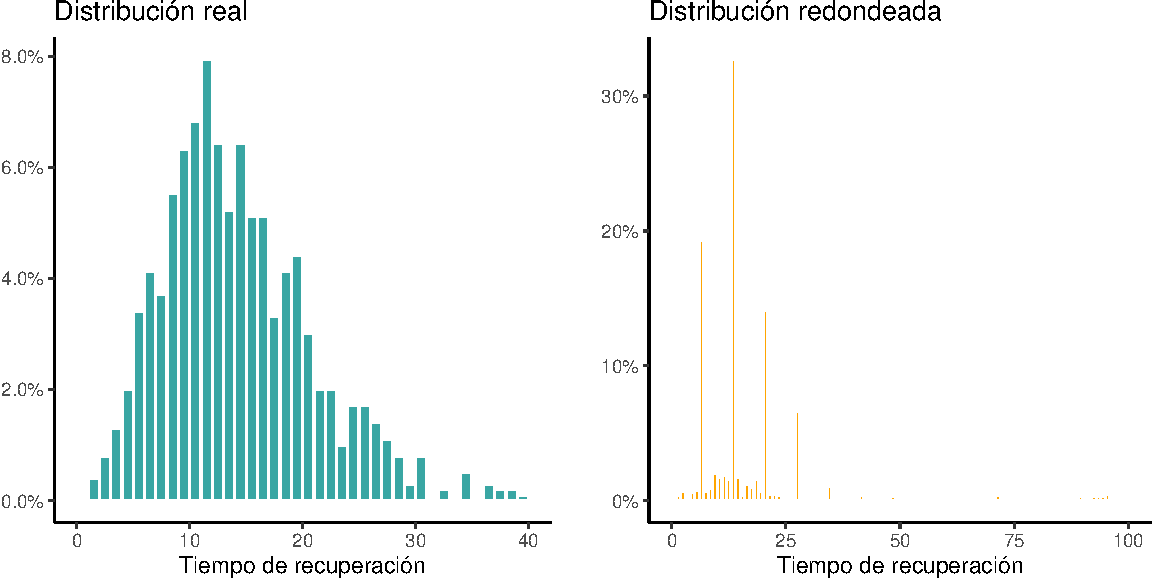
\includegraphics{Nota_Metodologica_v1_files/figure-latex/unnamed-chunk-1-1} \end{center}

En los datos observados (gráfica derecha) se modificaron, además, al 5\%
de los valores a fin de generar observaciones atípicas de ahí que la
gráfica amarilla aparezca con un mayor sesgo a la derecha y valores
cercanos a 100. Esto para reflejar de mejor mandera los datos reales.

El modelo funciona como sigue: para cada padecimiento, grupo de edad y
sexo, se supone que una proporción (desconocida) de los datos
corresponderá a atípicos. Para cada uno de los datos se analiza
\emph{qué es lo más probable}: que el valor sea atípico o que
corresponda a los datos reales. Esto permite generar dos bases
distintas: las de los probablemente atípicos y la de los probablemente
reales. Sobre la base de aquellos clasificados como probablemente reales
se busca entonces la mejor distribución de probabilidad que, al momento
de muestrear de ella y redondear los resultados, se obtengan
observaciones similares a los datos observados. Este proceso se repite
múltiples veces para garantizar que los resultados no se deban sólo al
azar.

De manera resumida el proceso está dado por:

\begin{enumerate}
\def\labelenumi{\arabic{enumi}.}
\item
  Clasificar (de manera aleatoria) algunos de los datos como atípicos.
\item
  Ajustar un modelo de probabilidad a los datos restantes de tal forma
  que, al redondear de dicho modelo, se obtengan los resultados más
  parecidos posibles a lo observado.
\item
  Repetir.
\end{enumerate}

La siguiente gráfica, resultante de simulaciones (ver más abajo),
muestra bajo una base de datos sintética cómo se ve la verdadera
distribución de los datos (\emph{real}), cómo resultan los datos
observados a partir de ella (\emph{redondeado}) y cómo ajusta el modelo
resultante de los pasos anteriores (\emph{modelo}). Dicha base de datos
sintética contiene además un 5\% valores atípicos en la derecha que el
modelo, adecuadamente, decide no ajustar.

\begin{figure}
\centering
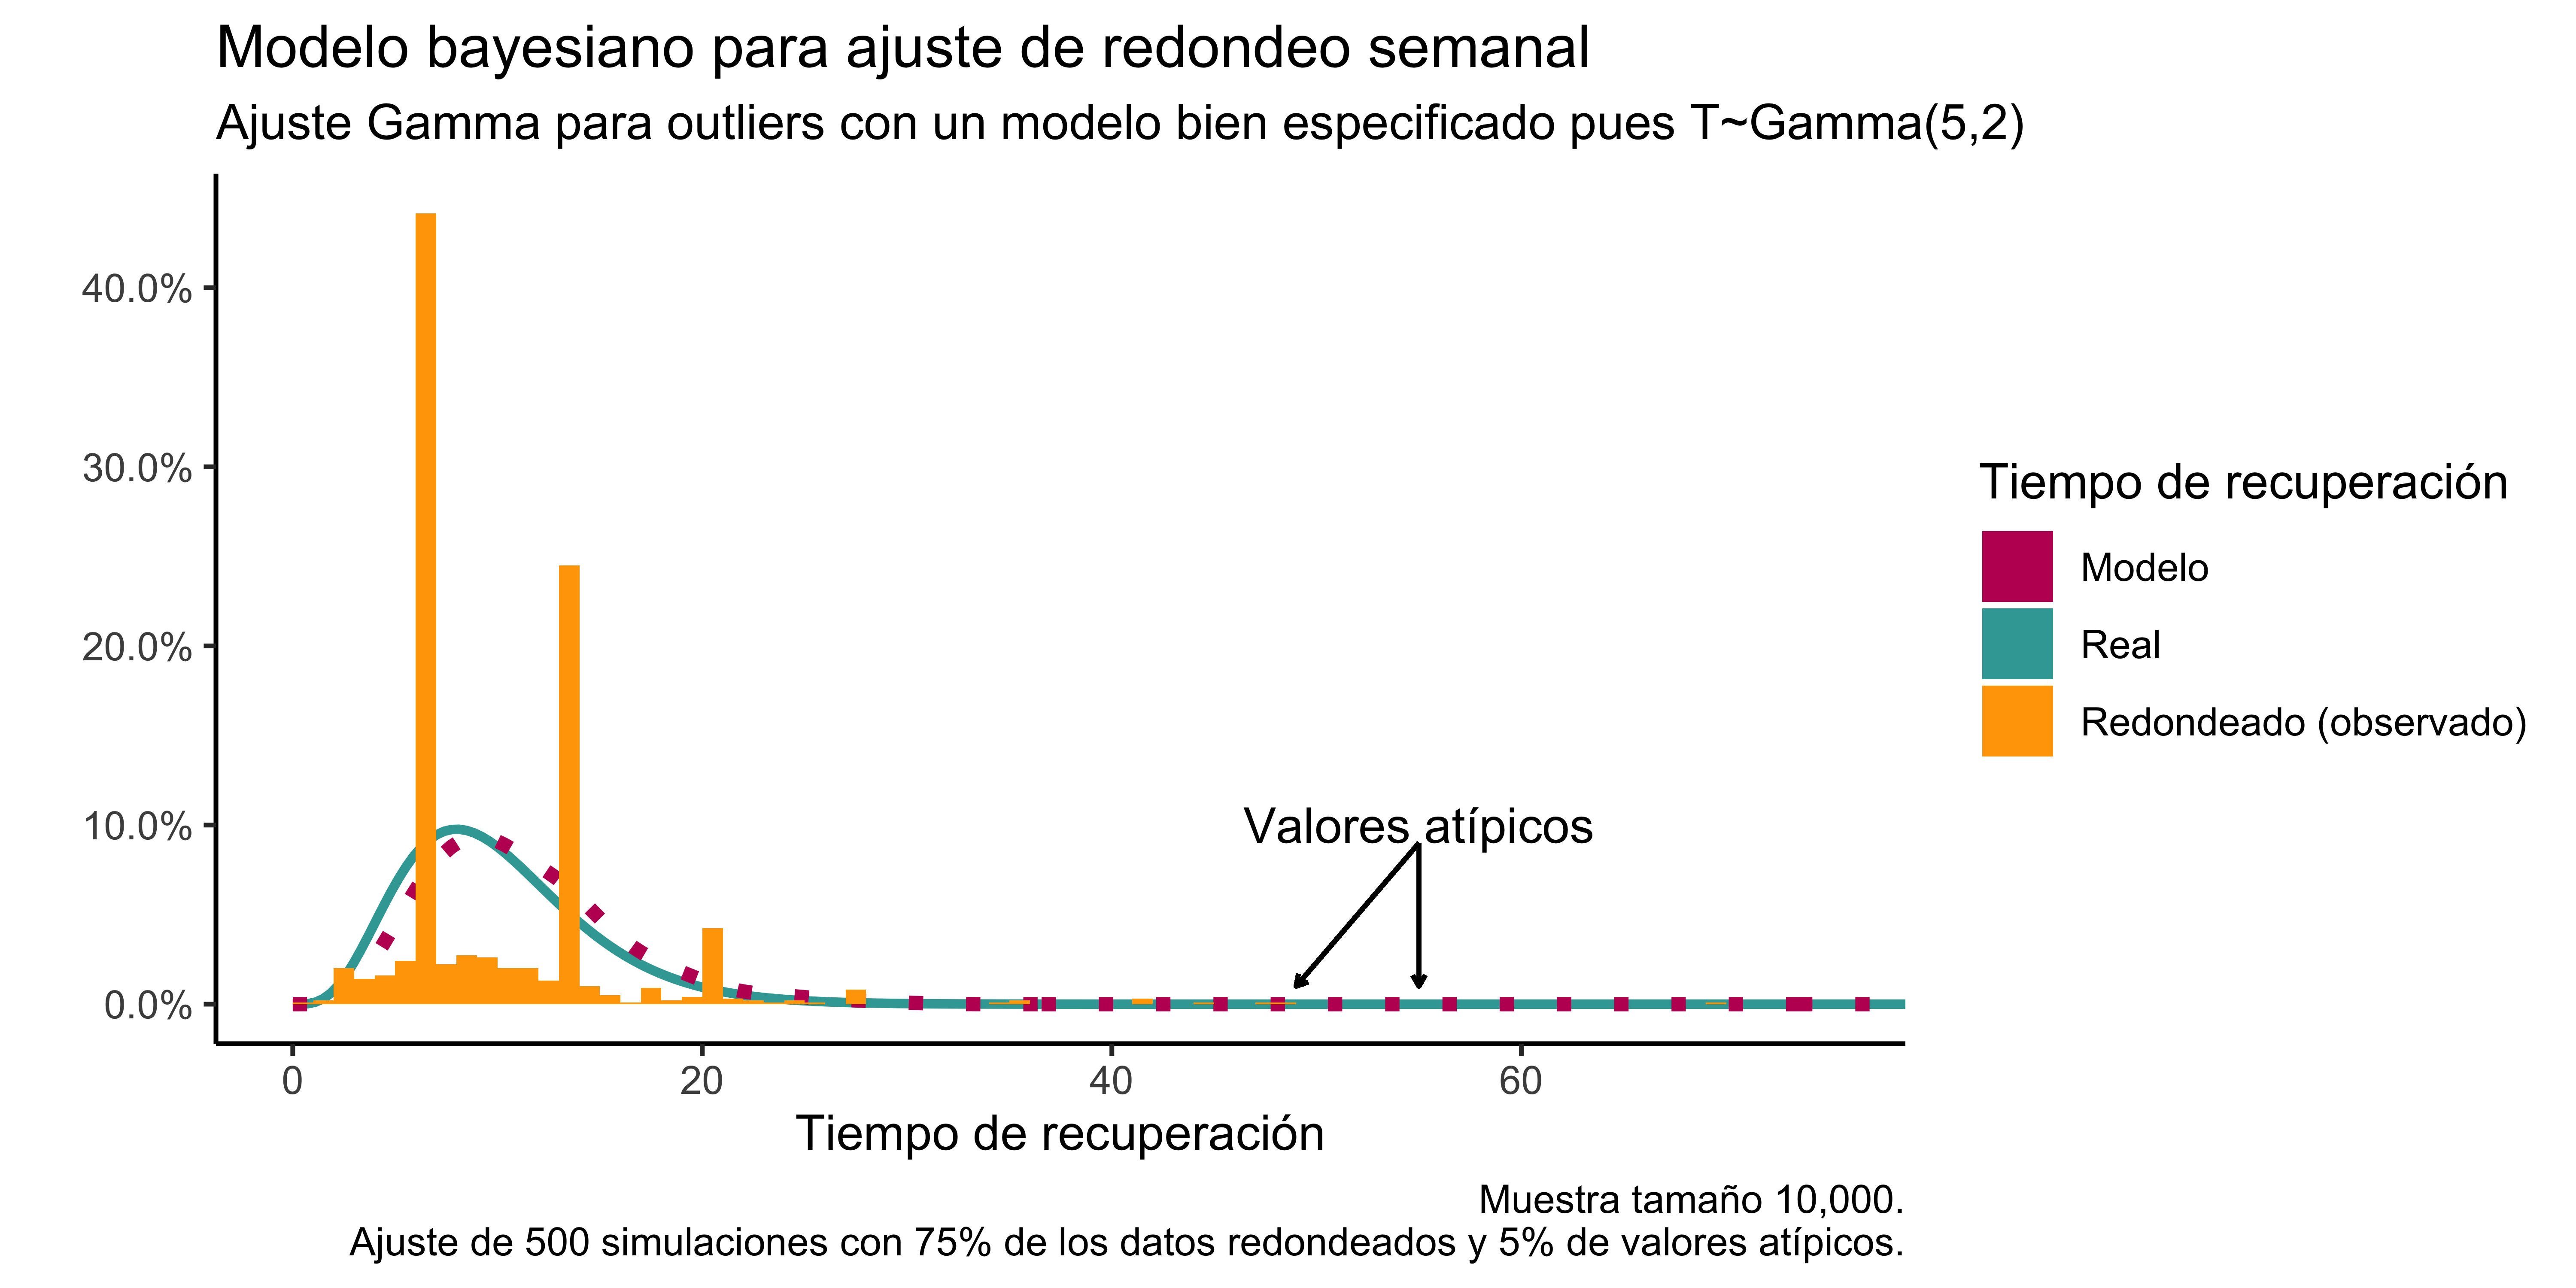
\includegraphics{images/Atipicosgamma.png}
\caption{Distribución redondeada con valores atípicos. Comparativo con
modelo original y modelo estimado.}
\end{figure}

El modelo que aquí se presenta es una adaptación del modelo de variables
latentes para redondeo de Gelman \emph{et al} (CITAR).

\hypertarget{ajuste-simple}{%
\subsubsection{Ajuste simple}\label{ajuste-simple}}

\begin{quote}
Ésta es una explicación más sencilla del ajuste que el modelo completo
pues no considera edad ni sexo.
\end{quote}

Para cada paciente \(i\), sea \(T^{R}_i\) el tiempo prescrito por el
médico ya con redondeo. Dicho tiempo está en función del verdadero
tiempo de recuperación (desconocido), \(T_i\): \[
T^{R}_i = T_i + \epsilon_i
\] donde \(\epsilon_i\) es el error de redondeo. Si \(\epsilon_i = 0\)
no hay redondeo en los datos y los observados corresponden a los
teóricos. Una cierta proporción de los tiempos observados son en
realidad valores atípicos. A estos, los denotamos \(T_i^{A}\) y
suponemos que: \[
T_i^{A} = \mathcal{O}_i + \zeta_i
\] donde \(\mathcal{O}_i\) es la distribución de los atípicos y
\(\zeta_i\) su error asociado.

Para cada paciente se observa un valor en la base \(T_i^{obs}\), el
cual, con probabilidad \(1 - \theta\) es un valor atípico: \[
T_i^{obs} = \begin{cases}
T_i^{R} & \textrm{ con probabilidad } \theta, \\
T_i^{A} & \textrm{ con probabilidad } 1 - \theta. \\
\end{cases}
\] El ajuste se realiza de manera bayesiana donde se supone:
\begin{equation}
\begin{aligned}
\theta & \sim \textrm{Beta}(0.25,1) \\
T_i|\alpha_R,\beta_R          & \sim \textrm{Gamma}(\alpha_R, \beta_R), \\
\mathcal{O}_i|\alpha_A,\beta_A & \sim \textrm{Gamma}(\alpha_A, \beta_A),
\end{aligned}
\end{equation} donde
\(\alpha_k, \beta_j \sim \textrm{HalfCauchy}(0, 2.5)\) para
\(k,j \in \{R,A\}\). Se tienen además las siguientes identidades que
relacionan los datos observados con el modelo teórico: \begin{equation}
\begin{aligned}
T_i & = T_i^{R} + \epsilon_i, \\
\mathcal{O}_i & = T_i^{A} + \zeta_i. \\
\end{aligned}
\end{equation} donde \(\epsilon_i\sim\textrm{Uniforme}(-3.5,3.5)\) es el
error de redondeo semanal y \(\zeta_i\sim\textrm{Uniforme}(0,1000)\) es
el error correspondiente a un valor atípico.

El modelo puede ser ajustado en \texttt{Stan} de la siguiente forma:

\begin{verbatim}
data {
  int<lower=0> N;
  vector[N] Tobs;
}

parameters {
  real<lower=0> alpha[2];
  real<lower=0> beta[2];
  real<lower=0, upper=1> theta;
  vector<lower=-3.5, upper=3.5>[N] error1;
  vector<lower=0, upper=1000>[N] error2;
}

transformed parameters {
  vector[N] Treal;
  vector[N] Outlier;
  Treal   = Tobs + error1; 
  Outlier = Tobs + error2; 
}

model {
  alpha    ~ cauchy(0, 2.5);
  beta     ~ cauchy(0, 2.5);
  error1   ~ uniform(-3.5, 3.5);
  error2   ~ uniform(0, 1000);
  theta    ~ beta(0.25,1);
  for (n in 1:N)
  target += log_mix(theta,
                    gamma_lpdf(Treal[n] | alpha[1], beta[1]),
                    gamma_lpdf(Outlier[n] | alpha[2], beta[2]));
}

generated quantities {
  real Tpred       = gamma_rng(alpha[1], beta[1]);
  real Outlierpred = gamma_rng(alpha[2], beta[2]);
}
\end{verbatim}

La siguiente gráfica muestra que incluso si especificamos de manera
incorrecta la distribución a priori de \(T_i^{R}\) tomándola como
Weibull en lugar de Gamma, el modelo de todas maneras ajusta
correctamente si \(n\) es relativamente grande:

\begin{figure}
\centering
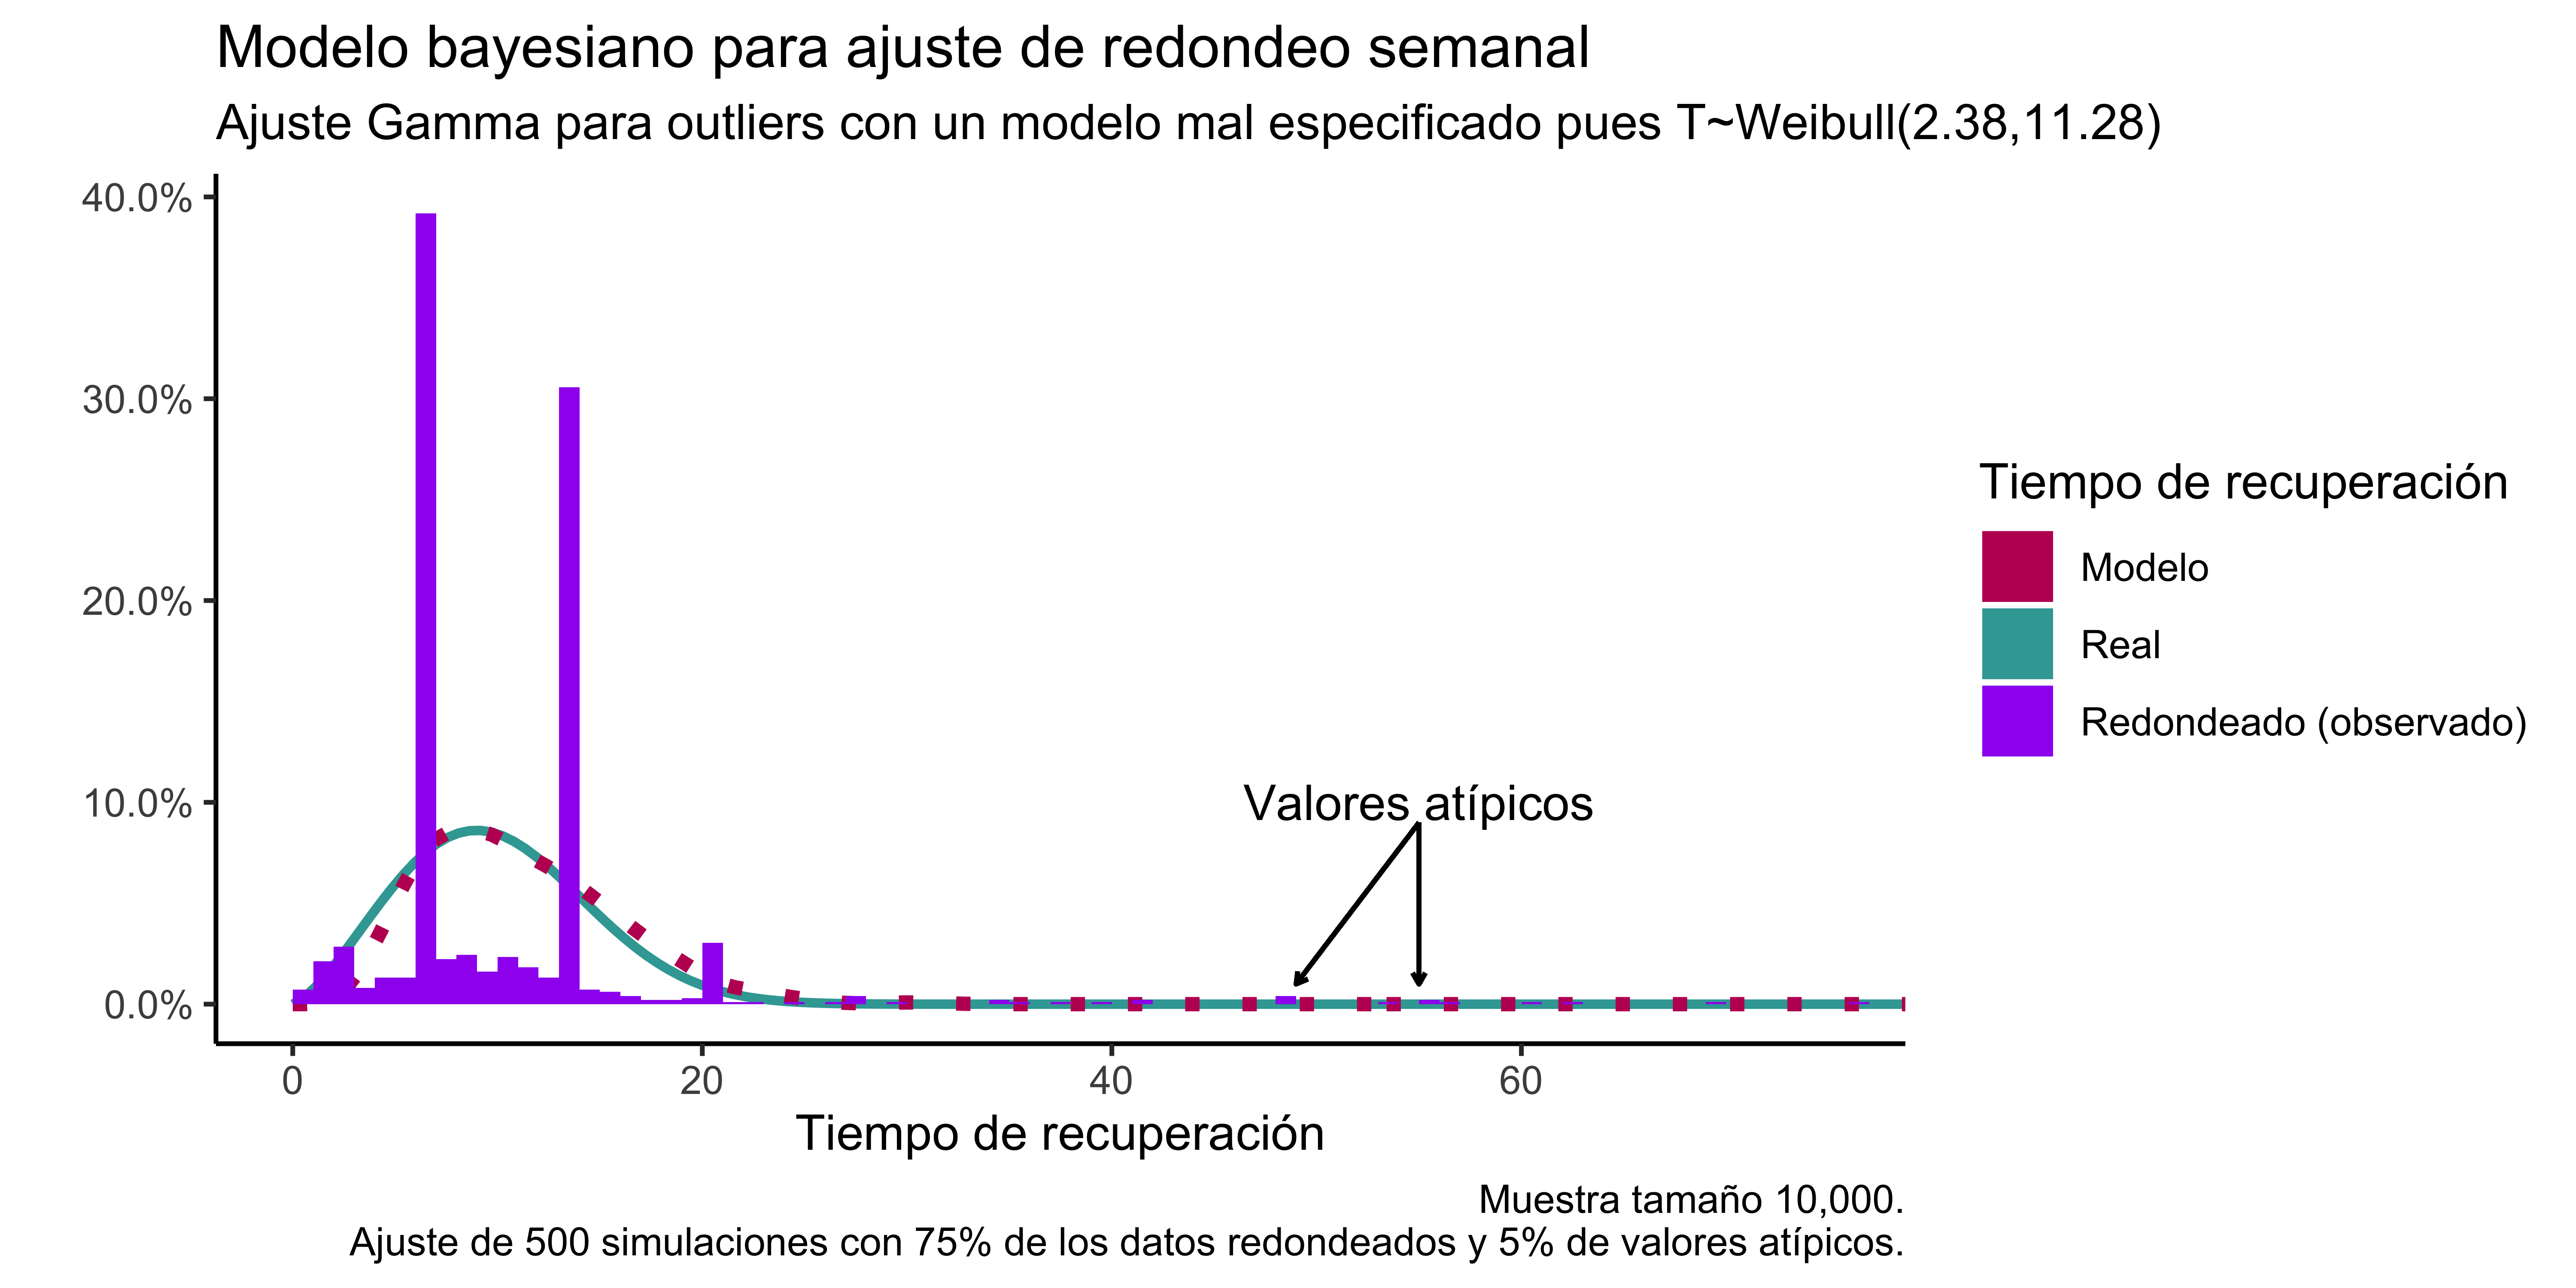
\includegraphics{images/Atipicosweibull.png}
\caption{Distribución redondeada con valores atípicos especificando de
manera incorrecta la distribución a priori. Comparativo con modelo
original y modelo estimado.}
\end{figure}

Código de \texttt{R} para generar datos que sigan esta distribución y
validar el modelo puede encontrarse en el apéndice.

\hypertarget{ajuste-controlando-por-edad-sexo-y-enfermedad.}{%
\subsubsection{Ajuste controlando por edad, sexo y
enfermedad.}\label{ajuste-controlando-por-edad-sexo-y-enfermedad.}}

Para el ajuste por sexo y edad, para cada enfermedad se establece una
regresión donde la media de tiempo de recuperación (\(\mu_R\)) es de la
forma: \[
\mu_R = \nu_R + \gamma_R\cdot\textrm{Edad}_i + \eta_R\cdot\textrm{Sexo}_i, 
\] mientras que la media de la distribución de valores atípicos está
dada por \[
\mu_A = \nu_A + \gamma_A\cdot\textrm{Edad}_i + \eta_A\cdot\textrm{Sexo}_i.   
\] En ambos casos se tiene la parametrización anterior: \begin{equation}
\begin{aligned}
T_i|\alpha_R,\beta_R          & \sim \textrm{Gamma}(\alpha_R, \beta_R), \\
\mathcal{O}_i|\alpha_A,\beta_A & \sim \textrm{Gamma}(\alpha_A, \beta_A),
\end{aligned}
\end{equation} donde \[
\alpha_j = \mu_j/\beta_j
\] para \(j \in\{A,R\}\). Las distribuciones \emph{a priori} de los
nuevos parámetros son: \begin{equation}
\begin{aligned}
\nu_j, \beta_j & \sim \textrm{HalfCauchy}(0, 2.5),\\
\gamma_j, \eta_j & \sim \textrm{Normal}(0,10000).
\end{aligned}
\end{equation} para \(k,j \in \{R,A\}\).

El modelo puede ser ajustado en \texttt{Stan} de la siguiente forma:

\begin{verbatim}
data {
  int<lower=0> N;
  vector[N] Tobs;
  vector[N] Edad;
  vector[N] Sexo;
  
  //Edades a interpolar en el resultado para reporte
  int<lower=0> M; 
  vector[M] EdadesResultado; 
}

parameters {
  vector[2] gamma;
  vector[2] eta;
  vector<lower=0>[2] nu;
  vector<lower=0>[2] beta;
  
  //Probability of outlier
  real<lower=0, upper=1> theta;
  
  //Roundong and outlier error as params (latent variables)
  vector<lower=-3.5, upper=3.5>[N] error1;
  vector<lower=0, upper=1000>[N] error2;
}

transformed parameters {
  vector[N] Treal;
  vector[N] Outlier;
  vector[N] mu_real;
  vector[N] mu_outlier;
  
  //Parámetro de medias de la regresión
  mu_real    = nu[1] + gamma[1]*Edad + eta[1]* Sexo;
  mu_outlier = nu[2] + gamma[2]*Edad + eta[2]* Sexo;
  
  //Datos con redondeo en función de los observados
  Treal   = Tobs + error1; 
  Outlier = Tobs + error2; 
}

model {
  nu       ~ cauchy(0, 2.5);
  beta     ~ cauchy(0, 2.5);
  gamma    ~ normal(0, 1000);
  eta      ~ normal(0, 1000);
  error1   ~ uniform(-3.5, 3.5);
  error2   ~ uniform(0, 1000);
  theta    ~ beta(0.25,1);
  for (n in 1:N)
  target += log_mix(theta,
                    gamma_lpdf(Treal[n] | mu_real[n] / beta[1], beta[1]),
                    gamma_lpdf(Outlier[n] | mu_outlier[n] / beta[2], beta[2]));
}

generated quantities {
  
  vector[M] Tpred_0;
  vector[M] Tpred_1;
  vector[M] Outlierpred_0;
  vector[M] Outlierpred_1;
  real mu_real_pred_0;
  real mu_real_pred_1;
  real mu_outlier_pred_0;
  real mu_outlier_pred_1;
  
  for (m in 1:M){
    //Sims
    mu_real_pred_0    = nu[1] + gamma[1]*EdadesResultado[m];
    mu_real_pred_1    = nu[1] + gamma[1]*EdadesResultado[m] + eta[1];
    mu_outlier_pred_0 = nu[2] + gamma[2]*EdadesResultado[m];
    mu_outlier_pred_1 = nu[2] + gamma[2]*EdadesResultado[m] + eta[2];
  
    Tpred_0[m]         = gamma_rng(mu_real_pred_0 ./ beta[1], beta[1]);
    Tpred_1[m]         = gamma_rng(mu_real_pred_1 ./ beta[1], beta[1]);
    Outlierpred_0[m]   = gamma_rng(mu_outlier_pred_0 ./ beta[2], beta[2]);
    Outlierpred_1[m]   = gamma_rng(mu_outlier_pred_1 ./ beta[2], beta[2]);
  }
}
\end{verbatim}

El ajuste con datos redondeados se ve de la siguiente manera. Cabe
recordar que el modelo opera conociendo sólo los datos que provienen del
redondeo y desconoce la distribución real.

\begin{figure}
\centering
\includegraphics{images/Atipicos_edad_gamma.png}
\caption{Ajuste de datos redondeados mediante modelo Gamma bayesiano
controlando por sexo y edad. Comparativo con modelo original y modelo
estimado usando sólo datos redondeados a múltiplos de 7.}
\end{figure}

El código de \texttt{R} para generar datos que sigan esta distribución y
validar el modelo puede encontrarse en el apéndice.

\hypertarget{apuxe9ndice}{%
\subsection{Apéndice}\label{apuxe9ndice}}

\hypertarget{cuxf3digo-de-r-para-generar-ajuste-simple}{%
\subsubsection{Código de R para generar ajuste
simple}\label{cuxf3digo-de-r-para-generar-ajuste-simple}}

El siguiente código genera datos que se comportan de acuerdo al modelo y
ajusta una distribución. Si la distribución de los datos coincide con la
distribución \emph{a priori} del modelo entonces el ajuste es perfecto.
Si la distribución no coincide de manera completa (por ejemplo teniendo
datos Weibull y un modelo Gamma) el ajuste de todas formas es muy bueno:

\begin{Shaded}
\begin{Highlighting}[]
\CommentTok{\#Script para simular la estructura de datos y verificar}
\CommentTok{\#si el modelo funciona para recuperarlos}
\FunctionTok{rm}\NormalTok{(}\AttributeTok{list =} \FunctionTok{ls}\NormalTok{())}

\FunctionTok{library}\NormalTok{(tidyverse)}
\FunctionTok{library}\NormalTok{(cmdstanr)}
\FunctionTok{library}\NormalTok{(scales)}
\FunctionTok{library}\NormalTok{(posterior)}
\FunctionTok{library}\NormalTok{(kdensity)}
\FunctionTok{library}\NormalTok{(bayesplot)}
\FunctionTok{library}\NormalTok{(mixdist)}

\FunctionTok{set.seed}\NormalTok{(}\DecValTok{23476785}\NormalTok{)}
\NormalTok{stan\_seed }\OtherTok{\textless{}{-}} \DecValTok{23749}
\NormalTok{chains }\OtherTok{=} \DecValTok{4}\NormalTok{; iter\_warmup }\OtherTok{=} \DecValTok{250}\NormalTok{; nsim }\OtherTok{=} \DecValTok{500}\NormalTok{; pchains }\OtherTok{=} \DecValTok{4}\NormalTok{; }
\NormalTok{threads\_per\_chain }\OtherTok{=} \DecValTok{4}\NormalTok{; threads }\OtherTok{=} \DecValTok{8}\NormalTok{; iter\_variational }\OtherTok{=} \DecValTok{10000}
\NormalTok{method }\OtherTok{=} \StringTok{"variational"} \CommentTok{\#faster (less accurate option) = "variational"}

\CommentTok{\#Flags for my compiler faster}
\NormalTok{compiler\_path\_cxx }\OtherTok{\textless{}{-}} \StringTok{"/usr/local/opt/llvm/bin/clang++"}
\FunctionTok{options}\NormalTok{(}\AttributeTok{mc.cores =}\NormalTok{ parallel}\SpecialCharTok{::}\FunctionTok{detectCores}\NormalTok{())}

\CommentTok{\#Simulation distribution}
\CommentTok{\#gamma para que el modelo esté bien especificado;}
\CommentTok{\#weibull para que no esté bien especificado}
\NormalTok{simdist }\OtherTok{\textless{}{-}} \StringTok{"gamma"} \CommentTok{\#weibull ó gamma}
\NormalTok{media    }\OtherTok{\textless{}{-}} \DecValTok{10}
\NormalTok{varianza }\OtherTok{\textless{}{-}} \DecValTok{20}

\CommentTok{\#No todos los datos están redondeados así que se establece un porcentaje}
\CommentTok{\#de cuántos tienen redondeo}
\NormalTok{perc\_redondeado }\OtherTok{\textless{}{-}} \FloatTok{0.75}  \CommentTok{\#Porcentaje de datos redondeados a 7}
\NormalTok{perc\_outliers   }\OtherTok{\textless{}{-}} \FloatTok{0.05}  \CommentTok{\#Se agrega el 1\% de outliers}
\NormalTok{nsims           }\OtherTok{\textless{}{-}} \DecValTok{10000} \CommentTok{\#Número de simulaciones para el modelo}

\CommentTok{\#Generamos las simulaciones:}
\ControlFlowTok{if}\NormalTok{ (simdist }\SpecialCharTok{==} \StringTok{"gamma"}\NormalTok{)\{}
  \FunctionTok{message}\NormalTok{(}\StringTok{"Distribución Gamma"}\NormalTok{)}
\NormalTok{  scale        }\OtherTok{\textless{}{-}}\NormalTok{ varianza}\SpecialCharTok{/}\NormalTok{media  }\SpecialCharTok{\%\textgreater{}\%} \FunctionTok{round}\NormalTok{(.,}\DecValTok{2}\NormalTok{)}
\NormalTok{  shape        }\OtherTok{\textless{}{-}}\NormalTok{ media}\SpecialCharTok{/}\NormalTok{scale     }\SpecialCharTok{\%\textgreater{}\%} \FunctionTok{round}\NormalTok{(.,}\DecValTok{2}\NormalTok{)}
\NormalTok{  col\_redondeo }\OtherTok{\textless{}{-}} \StringTok{"orange"}
\NormalTok{  tipo\_modelo  }\OtherTok{\textless{}{-}} \FunctionTok{paste0}\NormalTok{(}\StringTok{"bien especificado pues T\textasciitilde{}Gamma("}\NormalTok{, }
\NormalTok{                         shape, }\StringTok{","}\NormalTok{, scale,}\StringTok{")"}\NormalTok{)}
\NormalTok{  sample\_dist  }\OtherTok{\textless{}{-}} \ControlFlowTok{function}\NormalTok{()\{}\FunctionTok{rgamma}\NormalTok{(nsims, }\AttributeTok{shape =}\NormalTok{ shape, }\AttributeTok{scale =}\NormalTok{ scale)\}}
\NormalTok{  dist\_fun     }\OtherTok{\textless{}{-}} \ControlFlowTok{function}\NormalTok{(x)\{}\FunctionTok{dgamma}\NormalTok{(x, }\AttributeTok{shape =}\NormalTok{ shape, }\AttributeTok{scale =}\NormalTok{ scale)\}}
\NormalTok{\} }\ControlFlowTok{else} \ControlFlowTok{if}\NormalTok{ (simdist }\SpecialCharTok{==} \StringTok{"weibull"}\NormalTok{)\{}
  \FunctionTok{message}\NormalTok{(}\StringTok{"Distribución Weibull"}\NormalTok{)}
\NormalTok{  params       }\OtherTok{\textless{}{-}} \FunctionTok{weibullpar}\NormalTok{(media, }\FunctionTok{sqrt}\NormalTok{(varianza))}
\NormalTok{  shape        }\OtherTok{\textless{}{-}}\NormalTok{ params[}\StringTok{"shape"}\NormalTok{] }\SpecialCharTok{\%\textgreater{}\%} \FunctionTok{as.numeric}\NormalTok{() }\SpecialCharTok{\%\textgreater{}\%} \FunctionTok{round}\NormalTok{(.,}\DecValTok{2}\NormalTok{)}
\NormalTok{  scale        }\OtherTok{\textless{}{-}}\NormalTok{ params[}\StringTok{"scale"}\NormalTok{] }\SpecialCharTok{\%\textgreater{}\%} \FunctionTok{as.numeric}\NormalTok{() }\SpecialCharTok{\%\textgreater{}\%} \FunctionTok{round}\NormalTok{(.,}\DecValTok{2}\NormalTok{)}
\NormalTok{  col\_redondeo }\OtherTok{\textless{}{-}} \StringTok{"purple"}
\NormalTok{  tipo\_modelo  }\OtherTok{\textless{}{-}} \FunctionTok{paste0}\NormalTok{(}\StringTok{"mal especificado pues T\textasciitilde{}Weibull("}\NormalTok{, }
\NormalTok{                         shape, }\StringTok{","}\NormalTok{, scale,}\StringTok{")"}\NormalTok{)}
\NormalTok{  sample\_dist  }\OtherTok{\textless{}{-}} \ControlFlowTok{function}\NormalTok{(x)\{}\FunctionTok{rweibull}\NormalTok{(nsims, }\AttributeTok{shape =}\NormalTok{ shape, }\AttributeTok{scale =}\NormalTok{ scale)\}}
\NormalTok{  dist\_fun     }\OtherTok{\textless{}{-}} \ControlFlowTok{function}\NormalTok{(x)\{}\FunctionTok{dweibull}\NormalTok{(x, }\AttributeTok{shape =}\NormalTok{ shape, }\AttributeTok{scale =}\NormalTok{ scale)\}}
\NormalTok{\} }\ControlFlowTok{else}\NormalTok{ \{}
  \FunctionTok{stop}\NormalTok{(}\StringTok{"Distribución inválida selecciona \textquotesingle{}gamma\textquotesingle{} o \textquotesingle{}weibull\textquotesingle{}."}\NormalTok{)}
\NormalTok{\}}

\CommentTok{\#Simulamos los verdaderos datos filtrados como días (enteros)}
\NormalTok{datos\_distribucion }\OtherTok{\textless{}{-}} \FunctionTok{sample\_dist}\NormalTok{()}
\NormalTok{datos\_distribucion }\OtherTok{\textless{}{-}} \FunctionTok{round}\NormalTok{(datos\_distribucion,}\DecValTok{0}\NormalTok{)}

\CommentTok{\#Agregamos outliers}
\NormalTok{outliers\_id }\OtherTok{\textless{}{-}} \FunctionTok{sample}\NormalTok{(}\DecValTok{1}\SpecialCharTok{:}\NormalTok{nsims, }\FunctionTok{ceiling}\NormalTok{(perc\_outliers}\SpecialCharTok{*}\NormalTok{nsims))}
\NormalTok{outliers    }\OtherTok{\textless{}{-}} \FunctionTok{exp}\NormalTok{(}\FunctionTok{rnorm}\NormalTok{(}\FunctionTok{ceiling}\NormalTok{(perc\_outliers}\SpecialCharTok{*}\NormalTok{nsims), }\FunctionTok{log}\NormalTok{(}\DecValTok{50}\NormalTok{), }\DecValTok{1}\NormalTok{))}
\NormalTok{datos\_distribucion[outliers\_id] }\OtherTok{\textless{}{-}}\NormalTok{ outliers}

\CommentTok{\#Redondeamos la mayoría de los datos a múltiplos de 7 a partir de 3}
\NormalTok{redondear   }\OtherTok{\textless{}{-}}\NormalTok{ datos\_distribucion[datos\_distribucion }\SpecialCharTok{\textgreater{}} \DecValTok{3}\NormalTok{]}
\NormalTok{a\_redondear }\OtherTok{\textless{}{-}} \FunctionTok{sample}\NormalTok{(}\FunctionTok{ceiling}\NormalTok{(perc\_redondeado}\SpecialCharTok{*}\FunctionTok{length}\NormalTok{(redondear)))}
\NormalTok{redondear[a\_redondear]                     }\OtherTok{\textless{}{-}} \FunctionTok{round}\NormalTok{(redondear[a\_redondear]}\SpecialCharTok{/}\DecValTok{7}\NormalTok{)}\SpecialCharTok{*}\DecValTok{7}
\NormalTok{datos\_distribucion[datos\_distribucion }\SpecialCharTok{\textgreater{}} \DecValTok{3}\NormalTok{] }\OtherTok{\textless{}{-}}\NormalTok{ redondear}

\CommentTok{\#Modelo}
\FunctionTok{message}\NormalTok{(}\StringTok{"Fitting model. Go grab a coffee this will take A LOT"}\NormalTok{)}
\ControlFlowTok{if}\NormalTok{ (}\SpecialCharTok{!}\FunctionTok{is.null}\NormalTok{(compiler\_path\_cxx))\{}
\NormalTok{  cpp\_options }\OtherTok{\textless{}{-}} \FunctionTok{list}\NormalTok{(}\AttributeTok{cxx\_flags =} \StringTok{"{-}O3 {-}march=native"}\NormalTok{, }
                      \AttributeTok{cxx =}\NormalTok{ compiler\_path\_cxx, }\AttributeTok{stan\_threads =} \ConstantTok{TRUE}\NormalTok{)}
\NormalTok{\} }\ControlFlowTok{else}\NormalTok{ \{}
\NormalTok{  cpp\_options }\OtherTok{\textless{}{-}} \FunctionTok{list}\NormalTok{(}\AttributeTok{cxx\_flags =} \StringTok{"{-}O3 {-}march=native"}\NormalTok{, }
                      \AttributeTok{stan\_threads =} \ConstantTok{TRUE}\NormalTok{)}
\NormalTok{\}}

\NormalTok{model\_gamma\_v1 }\OtherTok{\textless{}{-}} \FunctionTok{cmdstan\_model}\NormalTok{(}\StringTok{"models/Modelo\_Gamma\_Outliers.stan"}\NormalTok{,}
                                \AttributeTok{cpp\_options =}\NormalTok{ cpp\_options)}

\NormalTok{datos }\OtherTok{\textless{}{-}} \FunctionTok{list}\NormalTok{(}\AttributeTok{N =} \FunctionTok{length}\NormalTok{(datos\_distribucion), }\AttributeTok{Tobs =}\NormalTok{ datos\_distribucion)}

\NormalTok{initf2 }\OtherTok{\textless{}{-}} \ControlFlowTok{function}\NormalTok{(}\AttributeTok{chain\_id =} \DecValTok{1}\NormalTok{) \{}
  \FunctionTok{list}\NormalTok{(}\AttributeTok{error1       =} \FunctionTok{runif}\NormalTok{(}\FunctionTok{length}\NormalTok{(datos\_distribucion), }\DecValTok{0}\NormalTok{, }\FloatTok{3.5}\NormalTok{), }
       \AttributeTok{error2       =} \FunctionTok{runif}\NormalTok{(}\FunctionTok{length}\NormalTok{(datos\_distribucion), }\DecValTok{0}\NormalTok{, }\DecValTok{1000}\NormalTok{), }
       \AttributeTok{alpha        =} \FunctionTok{rnorm}\NormalTok{(}\DecValTok{2}\NormalTok{, }\FloatTok{2.5}\NormalTok{, }\DecValTok{1}\NormalTok{) }\SpecialCharTok{\%\textgreater{}\%} \FunctionTok{abs}\NormalTok{(),}
       \AttributeTok{beta         =} \FunctionTok{rnorm}\NormalTok{(}\DecValTok{2}\NormalTok{, }\FloatTok{2.5}\NormalTok{, }\DecValTok{1}\NormalTok{) }\SpecialCharTok{\%\textgreater{}\%} \FunctionTok{abs}\NormalTok{(),}
       \AttributeTok{theta        =} \FunctionTok{runif}\NormalTok{(}\DecValTok{1}\NormalTok{,}\DecValTok{0}\NormalTok{,}\DecValTok{1}\NormalTok{)}
\NormalTok{  )\}}
\NormalTok{init\_ll }\OtherTok{\textless{}{-}} \FunctionTok{lapply}\NormalTok{(}\DecValTok{1}\SpecialCharTok{:}\NormalTok{chains, }\ControlFlowTok{function}\NormalTok{(id) }\FunctionTok{initf2}\NormalTok{(}\AttributeTok{chain\_id =}\NormalTok{ id))}

\ControlFlowTok{if}\NormalTok{ (}\SpecialCharTok{!}\FunctionTok{dir.exists}\NormalTok{(}\StringTok{"cmdstan"}\NormalTok{))\{}\FunctionTok{dir.create}\NormalTok{(}\StringTok{"cmdstan"}\NormalTok{)\}}
\ControlFlowTok{if}\NormalTok{ (method }\SpecialCharTok{==} \StringTok{"HMC"}\NormalTok{)\{}
\NormalTok{  model\_sample }\OtherTok{\textless{}{-}}\NormalTok{ model\_gamma\_v1}\SpecialCharTok{$}\FunctionTok{sample}\NormalTok{(}\AttributeTok{data =}\NormalTok{ datos, }
                                        \AttributeTok{chains =}\NormalTok{ chains, }
                                        \AttributeTok{seed =}\NormalTok{ stan\_seed, }
                                        \AttributeTok{iter\_warmup =}\NormalTok{ iter\_warmup,}
                                        \AttributeTok{adapt\_delta =} \FloatTok{0.95}\NormalTok{, }
                                        \AttributeTok{iter\_sampling =}\NormalTok{ nsim }\SpecialCharTok{{-}}\NormalTok{ iter\_warmup,}
                                        \AttributeTok{init =}\NormalTok{ initf2,}
                                        \AttributeTok{output\_dir =} \StringTok{"cmdstan"}\NormalTok{, }
                                        \AttributeTok{max\_treedepth =} \DecValTok{2}\SpecialCharTok{\^{}}\NormalTok{(}\DecValTok{11}\NormalTok{),}
                                        \AttributeTok{threads\_per\_chain =}\NormalTok{ threads\_per\_chain)}
\NormalTok{\} }\ControlFlowTok{else} \ControlFlowTok{if}\NormalTok{ (method }\SpecialCharTok{==} \StringTok{"variational"}\NormalTok{)\{}
\NormalTok{  model\_sample }\OtherTok{\textless{}{-}}\NormalTok{ model\_gamma\_v1}\SpecialCharTok{$}\FunctionTok{variational}\NormalTok{(}\AttributeTok{data =}\NormalTok{ datos, }
                                        \AttributeTok{seed =}\NormalTok{ stan\_seed, }
                                        \AttributeTok{iter=}\NormalTok{ iter\_variational,}
                                        \AttributeTok{init =}\NormalTok{ initf2,}
                                        \AttributeTok{threads =}\NormalTok{ threads,}
                                        \AttributeTok{output\_dir =} \StringTok{"cmdstan"}\NormalTok{)}
\NormalTok{\} }\ControlFlowTok{else}\NormalTok{ \{}
  \FunctionTok{message}\NormalTok{(}\FunctionTok{paste0}\NormalTok{(}\StringTok{"Method "}\NormalTok{, method, }\StringTok{" not found. Try \textquotesingle{}HMC\textquotesingle{} or \textquotesingle{}variational\textquotesingle{}"}\NormalTok{))}
\NormalTok{\}}

\CommentTok{\# Herramienta de diagnósitco para verificar el ajuste}
\CommentTok{\#model\_sample$cmdstan\_diagnose()}

\CommentTok{\#Obtenemos la distribución posterior}
\NormalTok{ppdist    }\OtherTok{\textless{}{-}}\NormalTok{ model\_sample}\SpecialCharTok{$}\FunctionTok{draws}\NormalTok{(}\AttributeTok{variables=}\StringTok{"Tpred"}\NormalTok{) }\SpecialCharTok{\%\textgreater{}\%} \FunctionTok{as\_draws\_df}\NormalTok{()}
\NormalTok{prop\_true }\OtherTok{\textless{}{-}}\NormalTok{ model\_sample}\SpecialCharTok{$}\FunctionTok{draws}\NormalTok{(}\AttributeTok{variables=}\StringTok{"theta"}\NormalTok{) }\SpecialCharTok{\%\textgreater{}\%} \FunctionTok{summarise\_draws}\NormalTok{()}

\CommentTok{\#Ajustamos densidades para graficar}
\CommentTok{\#Si tenemos demasiados datos reducimos para la gráfica}
\ControlFlowTok{if}\NormalTok{ (nsims }\SpecialCharTok{\textgreater{}} \DecValTok{1000}\NormalTok{)\{datos\_distribucion }\OtherTok{\textless{}{-}} \FunctionTok{sample}\NormalTok{(datos\_distribucion, }\DecValTok{1000}\NormalTok{)\}}
\NormalTok{x             }\OtherTok{\textless{}{-}} \FunctionTok{seq}\NormalTok{(}\DecValTok{0}\NormalTok{, }\FunctionTok{max}\NormalTok{(datos\_distribucion), }\AttributeTok{length.out =} \DecValTok{1000}\NormalTok{) }
\NormalTok{densidad\_real }\OtherTok{\textless{}{-}} \ControlFlowTok{function}\NormalTok{(x)\{}\FunctionTok{dist\_fun}\NormalTok{(x)\}}
\NormalTok{densidad\_obs  }\OtherTok{\textless{}{-}} \FunctionTok{kdensity}\NormalTok{(datos\_distribucion, }\AttributeTok{kernel =} \StringTok{"gaussian"}\NormalTok{)}
\NormalTok{densidad\_pred }\OtherTok{\textless{}{-}} \FunctionTok{kdensity}\NormalTok{(ppdist}\SpecialCharTok{$}\NormalTok{Tpred }\SpecialCharTok{+} \FloatTok{0.01}\NormalTok{, }\AttributeTok{start =} \StringTok{"gamma"}\NormalTok{, }
                          \AttributeTok{kernel =} \StringTok{"gaussian"}\NormalTok{, }\AttributeTok{support =} \FunctionTok{c}\NormalTok{(}\DecValTok{0}\NormalTok{, }\ConstantTok{Inf}\NormalTok{))}

\CommentTok{\#Gráfica de los datos}
\FunctionTok{data.frame}\NormalTok{(}\AttributeTok{x =}\NormalTok{ x, }\AttributeTok{Real =} \FunctionTok{densidad\_real}\NormalTok{(x), }\AttributeTok{Observada =} \FunctionTok{densidad\_obs}\NormalTok{(x), }
           \AttributeTok{Predicha =} \FunctionTok{densidad\_pred}\NormalTok{(x)) }\SpecialCharTok{\%\textgreater{}\%}
\FunctionTok{ggplot}\NormalTok{() }\SpecialCharTok{+}
  \FunctionTok{geom\_line}\NormalTok{(}\FunctionTok{aes}\NormalTok{(}\AttributeTok{x =}\NormalTok{ x, }\AttributeTok{y =}\NormalTok{ Real, }\AttributeTok{color =} \StringTok{"Real"}\NormalTok{), }\AttributeTok{size =} \DecValTok{1}\NormalTok{) }\SpecialCharTok{+}
  \FunctionTok{geom\_line}\NormalTok{(}\FunctionTok{aes}\NormalTok{(}\AttributeTok{x =}\NormalTok{ x, }\AttributeTok{y =}\NormalTok{ Predicha, }\AttributeTok{color =} \StringTok{"Modelo"}\NormalTok{), }\AttributeTok{size =} \FloatTok{1.5}\NormalTok{,}
            \AttributeTok{linetype =} \StringTok{"dotted"}\NormalTok{) }\SpecialCharTok{+}
  \FunctionTok{geom\_histogram}\NormalTok{(}\FunctionTok{aes}\NormalTok{(}\AttributeTok{x =}\NormalTok{ x, }\AttributeTok{y =}\NormalTok{ ..density.., }\AttributeTok{fill =} \StringTok{"Redondeado (observado)"}\NormalTok{),}
                 \AttributeTok{breaks =} \FunctionTok{seq}\NormalTok{(}\DecValTok{0}\NormalTok{,}\DecValTok{100}\NormalTok{, }\AttributeTok{by =} \DecValTok{1}\NormalTok{), }
                 \AttributeTok{data =} \FunctionTok{data.frame}\NormalTok{(}\AttributeTok{x =}\NormalTok{ datos\_distribucion)) }\SpecialCharTok{+}
  \FunctionTok{annotate}\NormalTok{(}\StringTok{"text"}\NormalTok{, }\AttributeTok{x =} \DecValTok{55}\NormalTok{, }\AttributeTok{y =} \FloatTok{0.1}\NormalTok{, }\AttributeTok{label =} \StringTok{"Valores atípicos"}\NormalTok{) }\SpecialCharTok{+}
  \FunctionTok{geom\_segment}\NormalTok{(}\FunctionTok{aes}\NormalTok{(}\AttributeTok{x =} \DecValTok{55}\NormalTok{, }\AttributeTok{y =} \FloatTok{0.09}\NormalTok{, }\AttributeTok{xend =} \DecValTok{55}\NormalTok{, }\AttributeTok{yend =} \FloatTok{0.01}\NormalTok{),}
               \AttributeTok{arrow =} \FunctionTok{arrow}\NormalTok{(}\AttributeTok{length =} \FunctionTok{unit}\NormalTok{(}\FloatTok{0.1}\NormalTok{, }\StringTok{"cm"}\NormalTok{))) }\SpecialCharTok{+}
  \FunctionTok{geom\_segment}\NormalTok{(}\FunctionTok{aes}\NormalTok{(}\AttributeTok{x =} \DecValTok{55}\NormalTok{, }\AttributeTok{y =} \FloatTok{0.09}\NormalTok{, }\AttributeTok{xend =} \DecValTok{49}\NormalTok{, }\AttributeTok{yend =} \FloatTok{0.01}\NormalTok{),}
               \AttributeTok{arrow =} \FunctionTok{arrow}\NormalTok{(}\AttributeTok{length =} \FunctionTok{unit}\NormalTok{(}\FloatTok{0.1}\NormalTok{, }\StringTok{"cm"}\NormalTok{))) }\SpecialCharTok{+}
  \FunctionTok{theme\_classic}\NormalTok{() }\SpecialCharTok{+}
  \FunctionTok{scale\_color\_manual}\NormalTok{(}\StringTok{"Tiempo de recuperación"}\NormalTok{,}
                     \AttributeTok{values =} \FunctionTok{c}\NormalTok{(}\StringTok{"Modelo"} \OtherTok{=} \StringTok{"\#BF1363"}\NormalTok{,}
                                \StringTok{"Real"} \OtherTok{=} \StringTok{"\#39A6A3"}\NormalTok{,}
                                \StringTok{"Redondeado (observado)"} \OtherTok{=}\NormalTok{ col\_redondeo)) }\SpecialCharTok{+}
  \FunctionTok{scale\_fill\_manual}\NormalTok{(}\StringTok{"Tiempo de recuperación"}\NormalTok{,}
                    \AttributeTok{values =} \FunctionTok{c}\NormalTok{(}\StringTok{"Modelo"} \OtherTok{=} \StringTok{"\#BF1363"}\NormalTok{,}
                               \StringTok{"Real"} \OtherTok{=} \StringTok{"\#39A6A3"}\NormalTok{,}
                               \StringTok{"Redondeado (observado)"} \OtherTok{=}\NormalTok{ col\_redondeo)) }\SpecialCharTok{+}
  \FunctionTok{labs}\NormalTok{(}
    \AttributeTok{x =} \StringTok{"Tiempo de recuperación"}\NormalTok{, }
    \AttributeTok{y =} \StringTok{""}\NormalTok{,}
    \AttributeTok{title =} \StringTok{"Modelo bayesiano para ajuste de redondeo semanal"}\NormalTok{,}
    \AttributeTok{subtitle =} \FunctionTok{paste0}\NormalTok{(}\StringTok{"Ajuste Gamma para outliers con un modelo "}\NormalTok{, tipo\_modelo),}
    \AttributeTok{caption =} \FunctionTok{paste0}\NormalTok{(}\StringTok{"Muestra tamaño "}\NormalTok{, }\FunctionTok{comma}\NormalTok{(nsims), }\StringTok{".}\SpecialCharTok{\textbackslash{}n}\StringTok{Ajuste de "}\NormalTok{, }
                     \FunctionTok{comma}\NormalTok{(nsim), }\StringTok{" simulaciones con "}\NormalTok{,}
                     \FunctionTok{percent}\NormalTok{(perc\_redondeado), }\StringTok{" de los datos redondeados y "}\NormalTok{, }
                     \FunctionTok{percent}\NormalTok{(perc\_outliers), }\StringTok{" de valores atípicos."}\NormalTok{)}
\NormalTok{  ) }\SpecialCharTok{+}
  \FunctionTok{coord\_cartesian}\NormalTok{(}\AttributeTok{xlim =} \FunctionTok{c}\NormalTok{(}\DecValTok{0}\NormalTok{, }\DecValTok{75}\NormalTok{)) }\SpecialCharTok{+}
  \FunctionTok{scale\_y\_continuous}\NormalTok{(}\AttributeTok{labels =}\NormalTok{ scales}\SpecialCharTok{::}\NormalTok{percent)}
\FunctionTok{ggsave}\NormalTok{(}\FunctionTok{paste0}\NormalTok{(}\StringTok{"images/Atipicos"}\NormalTok{,simdist,}\StringTok{".png"}\NormalTok{), }\AttributeTok{width =} \DecValTok{8}\NormalTok{, }
       \AttributeTok{height =} \DecValTok{4}\NormalTok{, }\AttributeTok{dpi =} \DecValTok{750}\NormalTok{)}
\end{Highlighting}
\end{Shaded}

\hypertarget{cuxf3digo-de-r-para-generar-ajuste-por-edad-y-sexo}{%
\subsubsection{Código de R para generar ajuste por edad y
sexo}\label{cuxf3digo-de-r-para-generar-ajuste-por-edad-y-sexo}}

\begin{Shaded}
\begin{Highlighting}[]
\CommentTok{\#Script para simular la estructura de datos y verificar}
\CommentTok{\#si el modelo funciona para recuperarlos}
\FunctionTok{rm}\NormalTok{(}\AttributeTok{list =} \FunctionTok{ls}\NormalTok{())}

\FunctionTok{library}\NormalTok{(tidyverse)}
\FunctionTok{library}\NormalTok{(cmdstanr)}
\FunctionTok{library}\NormalTok{(scales)}
\FunctionTok{library}\NormalTok{(posterior)}
\FunctionTok{library}\NormalTok{(kdensity)}
\FunctionTok{library}\NormalTok{(bayesplot)}
\FunctionTok{library}\NormalTok{(mixdist)}

\FunctionTok{set.seed}\NormalTok{(}\DecValTok{23476785}\NormalTok{)}
\NormalTok{stan\_seed }\OtherTok{\textless{}{-}} \DecValTok{23749}
\NormalTok{chains }\OtherTok{=} \DecValTok{4}\NormalTok{; iter\_warmup }\OtherTok{=} \DecValTok{250}\NormalTok{; nsim }\OtherTok{=} \DecValTok{500}\NormalTok{; pchains }\OtherTok{=} \DecValTok{4}\NormalTok{; }
\NormalTok{threads\_per\_chain }\OtherTok{=} \DecValTok{4}\NormalTok{; threads }\OtherTok{=} \DecValTok{12}\NormalTok{; iter\_variational }\OtherTok{=} \DecValTok{50000}\NormalTok{;}
\NormalTok{adapt\_iter }\OtherTok{=} \DecValTok{1000}\NormalTok{;}
\NormalTok{method }\OtherTok{=} \StringTok{"variational"} \CommentTok{\#faster (less accurate option) = "variational"}

\CommentTok{\#Flags for my compiler faster}
\NormalTok{compiler\_path\_cxx }\OtherTok{\textless{}{-}} \StringTok{"/usr/local/opt/llvm/bin/clang++"}
\FunctionTok{options}\NormalTok{(}\AttributeTok{mc.cores =}\NormalTok{ parallel}\SpecialCharTok{::}\FunctionTok{detectCores}\NormalTok{())}

\CommentTok{\#Simulation distribution}
\CommentTok{\#gamma para que el modelo esté bien especificado;}
\CommentTok{\#weibull para que no esté bien especificado}
\NormalTok{simdist }\OtherTok{\textless{}{-}} \StringTok{"gamma"} \CommentTok{\#weibull ó gamma}
\NormalTok{media\_baseline }\OtherTok{\textless{}{-}} \DecValTok{5}
\NormalTok{varianza       }\OtherTok{\textless{}{-}} \DecValTok{10}
\NormalTok{gamma\_edad     }\OtherTok{\textless{}{-}} \FloatTok{0.1}
\NormalTok{beta\_sexo      }\OtherTok{\textless{}{-}} \SpecialCharTok{{-}}\DecValTok{1}

\CommentTok{\#Edades a interpolar}
\NormalTok{edades\_interpol }\OtherTok{\textless{}{-}} \FunctionTok{c}\NormalTok{(}\DecValTok{30}\NormalTok{,}\DecValTok{40}\NormalTok{,}\DecValTok{50}\NormalTok{)}


\CommentTok{\#No todos los datos están redondeados así que se establece un porcentaje}
\CommentTok{\#de cuántos tienen redondeo}
\NormalTok{perc\_redondeado }\OtherTok{\textless{}{-}} \FloatTok{0.75}  \CommentTok{\#Porcentaje de datos redondeados a 7}
\NormalTok{perc\_outliers   }\OtherTok{\textless{}{-}} \FloatTok{0.05}  \CommentTok{\#Se agrega el 1\% de outliers}
\NormalTok{nsims           }\OtherTok{\textless{}{-}} \DecValTok{10000} \CommentTok{\#Número de simulaciones para el modelo}

\CommentTok{\#Simulamos las edades }
\NormalTok{edades }\OtherTok{\textless{}{-}} \FunctionTok{rnorm}\NormalTok{(nsims, }\AttributeTok{mean =} \DecValTok{40}\NormalTok{, }\AttributeTok{sd =} \DecValTok{10}\NormalTok{)}
\NormalTok{edades[(edades }\SpecialCharTok{\textless{}} \DecValTok{18} \SpecialCharTok{|}\NormalTok{ edades }\SpecialCharTok{\textgreater{}} \DecValTok{70}\NormalTok{)] }\OtherTok{\textless{}{-}} \FunctionTok{runif}\NormalTok{(}\FunctionTok{sum}\NormalTok{((edades }\SpecialCharTok{\textless{}} \DecValTok{18} \SpecialCharTok{|}\NormalTok{ edades }\SpecialCharTok{\textgreater{}} \DecValTok{70}\NormalTok{)), }\DecValTok{20}\NormalTok{, }\DecValTok{70}\NormalTok{)}

\CommentTok{\#Simulamos el sexo}
\NormalTok{psexo  }\OtherTok{\textless{}{-}} \FloatTok{0.4}
\NormalTok{sexo   }\OtherTok{\textless{}{-}} \FunctionTok{sample}\NormalTok{(}\FunctionTok{c}\NormalTok{(}\DecValTok{0}\NormalTok{,}\DecValTok{1}\NormalTok{), nsims, }\AttributeTok{replace =}\NormalTok{ T, }\AttributeTok{prob =} \FunctionTok{c}\NormalTok{(psexo, }\DecValTok{1}\SpecialCharTok{{-}}\NormalTok{psexo))}

\CommentTok{\#Generamos los parámetros}
\NormalTok{genera\_media }\OtherTok{\textless{}{-}} \ControlFlowTok{function}\NormalTok{(edad, sexo, }\AttributeTok{sims =}\NormalTok{ nsims, }\AttributeTok{random =}\NormalTok{ T)\{}
  \ControlFlowTok{if}\NormalTok{ (random)\{}
\NormalTok{    mu }\OtherTok{\textless{}{-}}\NormalTok{ media\_baseline }\SpecialCharTok{+} \FunctionTok{rnorm}\NormalTok{(sims, gamma\_edad, }\FloatTok{0.1}\NormalTok{)}\SpecialCharTok{*}\NormalTok{edad }\SpecialCharTok{+} \FunctionTok{rnorm}\NormalTok{(sims, beta\_sexo, }\FloatTok{0.1}\NormalTok{)}\SpecialCharTok{*}\NormalTok{sexo}
\NormalTok{    mu[mu }\SpecialCharTok{\textless{}} \DecValTok{0}\NormalTok{] }\OtherTok{\textless{}{-}}\NormalTok{ media\_baseline}
\NormalTok{  \} }\ControlFlowTok{else}\NormalTok{ \{}
\NormalTok{    mu }\OtherTok{\textless{}{-}}\NormalTok{ media\_baseline }\SpecialCharTok{+}\NormalTok{ gamma\_edad}\SpecialCharTok{*}\NormalTok{edad }\SpecialCharTok{+}\NormalTok{ beta\_sexo}\SpecialCharTok{*}\NormalTok{sexo}
\NormalTok{    mu[mu }\SpecialCharTok{\textless{}} \DecValTok{0}\NormalTok{] }\OtherTok{\textless{}{-}}\NormalTok{ media\_baseline}
\NormalTok{  \}}
  \FunctionTok{return}\NormalTok{(mu)}
\NormalTok{\}}
\NormalTok{media }\OtherTok{\textless{}{-}} \FunctionTok{genera\_media}\NormalTok{(edades, sexo)}

\ControlFlowTok{if}\NormalTok{ (}\FunctionTok{min}\NormalTok{(media }\SpecialCharTok{\textless{}} \DecValTok{0}\NormalTok{))\{}
  \FunctionTok{stop}\NormalTok{(}\StringTok{"Distribución no está bien especificada la media debe ser \textgreater{} 0"}\NormalTok{)}
\NormalTok{\}}

\CommentTok{\#Generamos las simulaciones:}
\ControlFlowTok{if}\NormalTok{ (simdist }\SpecialCharTok{==} \StringTok{"gamma"}\NormalTok{)\{}
  \FunctionTok{message}\NormalTok{(}\StringTok{"Distribución Gamma"}\NormalTok{)}
\NormalTok{  scale        }\OtherTok{\textless{}{-}}\NormalTok{ varianza}\SpecialCharTok{/}\NormalTok{media  }\SpecialCharTok{\%\textgreater{}\%} \FunctionTok{round}\NormalTok{(.,}\DecValTok{2}\NormalTok{)}
\NormalTok{  shape        }\OtherTok{\textless{}{-}}\NormalTok{ media}\SpecialCharTok{/}\NormalTok{scale     }\SpecialCharTok{\%\textgreater{}\%} \FunctionTok{round}\NormalTok{(.,}\DecValTok{2}\NormalTok{)}
\NormalTok{  col\_redondeo }\OtherTok{\textless{}{-}} \StringTok{"orange"}
\NormalTok{  tipo\_modelo  }\OtherTok{\textless{}{-}} \FunctionTok{paste0}\NormalTok{(}\StringTok{"bien especificado pues T\textasciitilde{}Gamma("}\NormalTok{, }
\NormalTok{                         shape, }\StringTok{","}\NormalTok{, scale,}\StringTok{")"}\NormalTok{)}
\NormalTok{  sample\_dist  }\OtherTok{\textless{}{-}} \ControlFlowTok{function}\NormalTok{()\{}
    \FunctionTok{rgamma}\NormalTok{(nsims, }\AttributeTok{shape =}\NormalTok{ shape, }\AttributeTok{scale =}\NormalTok{ scale)}
\NormalTok{  \}}
\NormalTok{  dist\_fun     }\OtherTok{\textless{}{-}} \ControlFlowTok{function}\NormalTok{(x, edad, sexo)\{}
\NormalTok{    scale }\OtherTok{\textless{}{-}}\NormalTok{ varianza}\SpecialCharTok{/}\FunctionTok{genera\_media}\NormalTok{(edad, sexo, }\DecValTok{1}\NormalTok{, }\AttributeTok{random =}\NormalTok{ F) }
\NormalTok{    shape }\OtherTok{\textless{}{-}} \FunctionTok{genera\_media}\NormalTok{(edad, sexo, }\DecValTok{1}\NormalTok{, }\AttributeTok{random =}\NormalTok{ F)}\SpecialCharTok{/}\NormalTok{scale}
    \FunctionTok{dgamma}\NormalTok{(x, }\AttributeTok{shape =}\NormalTok{ shape, }\AttributeTok{scale =}\NormalTok{ scale)}
\NormalTok{  \}}
\NormalTok{\} }\ControlFlowTok{else} \ControlFlowTok{if}\NormalTok{ (simdist }\SpecialCharTok{==} \StringTok{"weibull"}\NormalTok{)\{}
  \FunctionTok{message}\NormalTok{(}\StringTok{"Distribución Weibull"}\NormalTok{)}
\NormalTok{  params       }\OtherTok{\textless{}{-}} \FunctionTok{weibullpar}\NormalTok{(media, }\FunctionTok{sqrt}\NormalTok{(varianza))}
\NormalTok{  shape        }\OtherTok{\textless{}{-}}\NormalTok{ params[}\StringTok{"shape"}\NormalTok{]  }\SpecialCharTok{\%\textgreater{}\%} \FunctionTok{round}\NormalTok{(.,}\DecValTok{2}\NormalTok{)}
\NormalTok{  scale        }\OtherTok{\textless{}{-}}\NormalTok{ params[}\StringTok{"scale"}\NormalTok{]  }\SpecialCharTok{\%\textgreater{}\%} \FunctionTok{round}\NormalTok{(.,}\DecValTok{2}\NormalTok{)}
\NormalTok{  col\_redondeo }\OtherTok{\textless{}{-}} \StringTok{"purple"}
\NormalTok{  tipo\_modelo  }\OtherTok{\textless{}{-}} \FunctionTok{paste0}\NormalTok{(}\StringTok{"mal especificado pues T\textasciitilde{}Weibull"}\NormalTok{)}
\NormalTok{  sample\_dist  }\OtherTok{\textless{}{-}} \ControlFlowTok{function}\NormalTok{(x)\{}
    \FunctionTok{rweibull}\NormalTok{(nsims, }\AttributeTok{shape =} \FunctionTok{unlist}\NormalTok{(shape), }\AttributeTok{scale =}  \FunctionTok{unlist}\NormalTok{(scale))}
\NormalTok{  \}}
\NormalTok{  dist\_fun     }\OtherTok{\textless{}{-}} \ControlFlowTok{function}\NormalTok{(x, edad, sexo)\{}
\NormalTok{    params       }\OtherTok{\textless{}{-}} \FunctionTok{weibullpar}\NormalTok{(}\FunctionTok{genera\_media}\NormalTok{(edad,sexo, }\DecValTok{1}\NormalTok{, }\AttributeTok{random =}\NormalTok{ F), }\FunctionTok{sqrt}\NormalTok{(varianza))}
\NormalTok{    shape        }\OtherTok{\textless{}{-}}\NormalTok{ params[}\StringTok{"shape"}\NormalTok{] }\SpecialCharTok{\%\textgreater{}\%} \FunctionTok{round}\NormalTok{(.,}\DecValTok{2}\NormalTok{)}
\NormalTok{    scale        }\OtherTok{\textless{}{-}}\NormalTok{ params[}\StringTok{"scale"}\NormalTok{] }\SpecialCharTok{\%\textgreater{}\%} \FunctionTok{round}\NormalTok{(.,}\DecValTok{2}\NormalTok{)}
    \FunctionTok{dweibull}\NormalTok{(x, }\AttributeTok{shape =} \FunctionTok{unlist}\NormalTok{(shape), }\AttributeTok{scale =} \FunctionTok{unlist}\NormalTok{(scale))}
\NormalTok{  \}}
\NormalTok{\} }\ControlFlowTok{else}\NormalTok{ \{}
  \FunctionTok{stop}\NormalTok{(}\StringTok{"Distribución inválida selecciona \textquotesingle{}gamma\textquotesingle{} o \textquotesingle{}weibull\textquotesingle{}."}\NormalTok{)}
\NormalTok{\}}


\CommentTok{\#Simulamos los verdaderos datos filtrados como días (enteros)}
\NormalTok{datos\_distribucion }\OtherTok{\textless{}{-}} \FunctionTok{sample\_dist}\NormalTok{()}
\NormalTok{datos\_distribucion }\OtherTok{\textless{}{-}} \FunctionTok{round}\NormalTok{(datos\_distribucion,}\DecValTok{0}\NormalTok{)}

\CommentTok{\#Agregamos outliers}
\NormalTok{outliers\_id }\OtherTok{\textless{}{-}} \FunctionTok{sample}\NormalTok{(}\DecValTok{1}\SpecialCharTok{:}\NormalTok{nsims, }\FunctionTok{ceiling}\NormalTok{(perc\_outliers}\SpecialCharTok{*}\NormalTok{nsims))}
\NormalTok{outliers    }\OtherTok{\textless{}{-}} \FunctionTok{exp}\NormalTok{(}\FunctionTok{rnorm}\NormalTok{(}\FunctionTok{ceiling}\NormalTok{(perc\_outliers}\SpecialCharTok{*}\NormalTok{nsims), }\FunctionTok{log}\NormalTok{(}\DecValTok{50}\NormalTok{), }\DecValTok{1}\NormalTok{))}
\NormalTok{datos\_distribucion[outliers\_id] }\OtherTok{\textless{}{-}}\NormalTok{ outliers}

\CommentTok{\#Redondeamos la mayoría de los datos a múltiplos de 7 a partir de 3}
\NormalTok{redondear   }\OtherTok{\textless{}{-}}\NormalTok{ datos\_distribucion[datos\_distribucion }\SpecialCharTok{\textgreater{}} \DecValTok{3}\NormalTok{]}
\NormalTok{a\_redondear }\OtherTok{\textless{}{-}} \FunctionTok{sample}\NormalTok{(}\FunctionTok{ceiling}\NormalTok{(perc\_redondeado}\SpecialCharTok{*}\FunctionTok{length}\NormalTok{(redondear)))}
\NormalTok{redondear[a\_redondear]                     }\OtherTok{\textless{}{-}} \FunctionTok{round}\NormalTok{(redondear[a\_redondear]}\SpecialCharTok{/}\DecValTok{7}\NormalTok{)}\SpecialCharTok{*}\DecValTok{7}
\NormalTok{datos\_distribucion[datos\_distribucion }\SpecialCharTok{\textgreater{}} \DecValTok{3}\NormalTok{] }\OtherTok{\textless{}{-}}\NormalTok{ redondear}

\CommentTok{\#Modelo}
\FunctionTok{message}\NormalTok{(}\StringTok{"Fitting model. Go grab a coffee this will take A LOT"}\NormalTok{)}
\ControlFlowTok{if}\NormalTok{ (}\SpecialCharTok{!}\FunctionTok{is.null}\NormalTok{(compiler\_path\_cxx))\{}
\NormalTok{  cpp\_options }\OtherTok{\textless{}{-}} \FunctionTok{list}\NormalTok{(}\AttributeTok{cxx\_flags =} \StringTok{"{-}O3 {-}march=native"}\NormalTok{, }
                      \AttributeTok{cxx =}\NormalTok{ compiler\_path\_cxx, }\AttributeTok{stan\_threads =} \ConstantTok{TRUE}\NormalTok{)}
\NormalTok{\} }\ControlFlowTok{else}\NormalTok{ \{}
\NormalTok{  cpp\_options }\OtherTok{\textless{}{-}} \FunctionTok{list}\NormalTok{(}\AttributeTok{cxx\_flags =} \StringTok{"{-}O3 {-}march=native"}\NormalTok{, }
                      \AttributeTok{stan\_threads =} \ConstantTok{TRUE}\NormalTok{)}
\NormalTok{\}}

\NormalTok{model\_gamma\_v1 }\OtherTok{\textless{}{-}} \FunctionTok{cmdstan\_model}\NormalTok{(}\StringTok{"models/Modelo\_Gamma\_Outliers\_Edad.stan"}\NormalTok{,}
                                \AttributeTok{cpp\_options =}\NormalTok{ cpp\_options)}

\NormalTok{datos }\OtherTok{\textless{}{-}} \FunctionTok{list}\NormalTok{(}\AttributeTok{N =} \FunctionTok{length}\NormalTok{(datos\_distribucion), }
              \AttributeTok{Tobs =}\NormalTok{ datos\_distribucion, }\AttributeTok{Edad =}\NormalTok{ edades, }\AttributeTok{Sexo =}\NormalTok{ sexo,}
              \AttributeTok{EdadesResultado =}\NormalTok{ edades\_interpol, }\AttributeTok{M =} \FunctionTok{length}\NormalTok{(edades\_interpol))}

\NormalTok{initf2 }\OtherTok{\textless{}{-}} \ControlFlowTok{function}\NormalTok{(}\AttributeTok{chain\_id =} \DecValTok{1}\NormalTok{) \{}
  \FunctionTok{list}\NormalTok{(}\AttributeTok{error1       =} \FunctionTok{runif}\NormalTok{(}\FunctionTok{length}\NormalTok{(datos\_distribucion), }\DecValTok{0}\NormalTok{, }\FloatTok{3.5}\NormalTok{), }
       \AttributeTok{error2       =} \FunctionTok{runif}\NormalTok{(}\FunctionTok{length}\NormalTok{(datos\_distribucion), }\DecValTok{0}\NormalTok{, }\DecValTok{1000}\NormalTok{), }
       \AttributeTok{beta         =}\NormalTok{ (}\FunctionTok{rnorm}\NormalTok{(}\DecValTok{2}\NormalTok{, }\FloatTok{2.5}\NormalTok{, }\DecValTok{1}\NormalTok{) }\SpecialCharTok{\%\textgreater{}\%} \FunctionTok{abs}\NormalTok{()) }\SpecialCharTok{+} \DecValTok{1}\NormalTok{,}
       \AttributeTok{gamma        =} \FunctionTok{rnorm}\NormalTok{(}\DecValTok{2}\NormalTok{, }\DecValTok{0}\NormalTok{, }\FloatTok{0.1}\NormalTok{),}
       \AttributeTok{eta          =} \FunctionTok{rnorm}\NormalTok{(}\DecValTok{2}\NormalTok{, }\DecValTok{0}\NormalTok{, }\FloatTok{0.1}\NormalTok{),}
       \AttributeTok{nu           =} \FunctionTok{rnorm}\NormalTok{(}\DecValTok{2}\NormalTok{, }\DecValTok{100}\NormalTok{, }\FloatTok{0.1}\NormalTok{) }\SpecialCharTok{\%\textgreater{}\%} \FunctionTok{abs}\NormalTok{(),}
       \AttributeTok{theta        =} \FunctionTok{runif}\NormalTok{(}\DecValTok{1}\NormalTok{,}\DecValTok{0}\NormalTok{,}\DecValTok{1}\NormalTok{)}
\NormalTok{  )\}}

\ControlFlowTok{if}\NormalTok{ (}\SpecialCharTok{!}\FunctionTok{dir.exists}\NormalTok{(}\StringTok{"cmdstan"}\NormalTok{))\{}\FunctionTok{dir.create}\NormalTok{(}\StringTok{"cmdstan"}\NormalTok{)\}}
\ControlFlowTok{if}\NormalTok{ (method }\SpecialCharTok{==} \StringTok{"HMC"}\NormalTok{)\{}
\NormalTok{  model\_sample }\OtherTok{\textless{}{-}}\NormalTok{ model\_gamma\_v1}\SpecialCharTok{$}\FunctionTok{sample}\NormalTok{(}\AttributeTok{data =}\NormalTok{ datos, }
                                        \AttributeTok{chains =}\NormalTok{ chains, }
                                        \AttributeTok{seed =}\NormalTok{ stan\_seed, }
                                        \AttributeTok{iter\_warmup =}\NormalTok{ iter\_warmup,}
                                        \AttributeTok{adapt\_delta =} \FloatTok{0.95}\NormalTok{, }
                                        \AttributeTok{iter\_sampling =}\NormalTok{ nsim }\SpecialCharTok{{-}}\NormalTok{ iter\_warmup,}
                                        \AttributeTok{init =}\NormalTok{ initf2,}
                                        \AttributeTok{output\_dir =} \StringTok{"cmdstan"}\NormalTok{, }
                                        \AttributeTok{max\_treedepth =} \DecValTok{2}\SpecialCharTok{\^{}}\NormalTok{(}\DecValTok{11}\NormalTok{),}
                                        \AttributeTok{threads\_per\_chain =}\NormalTok{ threads\_per\_chain)}
\NormalTok{\} }\ControlFlowTok{else} \ControlFlowTok{if}\NormalTok{ (method }\SpecialCharTok{==} \StringTok{"variational"}\NormalTok{)\{}
\NormalTok{  model\_sample }\OtherTok{\textless{}{-}}\NormalTok{ model\_gamma\_v1}\SpecialCharTok{$}\FunctionTok{variational}\NormalTok{(}\AttributeTok{data =}\NormalTok{ datos, }
                                             \AttributeTok{seed =}\NormalTok{ stan\_seed, }
                                             \AttributeTok{iter=}\NormalTok{ iter\_variational,}
                                             \AttributeTok{init =}\NormalTok{ initf2,}
                                             \AttributeTok{adapt\_iter =}\NormalTok{ adapt\_iter,}
                                             \AttributeTok{adapt\_engaged =}\NormalTok{ T,}
                                             \AttributeTok{output\_samples =} \DecValTok{1000}\NormalTok{,}
                                             \AttributeTok{threads =}\NormalTok{ threads,}
                                             \AttributeTok{output\_dir =} \StringTok{"cmdstan"}\NormalTok{)}
\NormalTok{\} }\ControlFlowTok{else}\NormalTok{ \{}
  \FunctionTok{message}\NormalTok{(}\FunctionTok{paste0}\NormalTok{(}\StringTok{"Method "}\NormalTok{, method, }\StringTok{" not found. Try \textquotesingle{}HMC\textquotesingle{} or \textquotesingle{}variational\textquotesingle{}"}\NormalTok{))}
\NormalTok{\}}

\CommentTok{\# Herramienta de diagnósitco para verificar el ajuste}
\CommentTok{\#model\_sample$cmdstan\_diagnose()}

\CommentTok{\#Obtenemos la distribución posterior}
\NormalTok{ppdist\_0  }\OtherTok{\textless{}{-}}\NormalTok{ model\_sample}\SpecialCharTok{$}\FunctionTok{draws}\NormalTok{(}\AttributeTok{variables=}\StringTok{"Tpred\_0"}\NormalTok{) }\SpecialCharTok{\%\textgreater{}\%} \FunctionTok{as\_draws\_df}\NormalTok{()}
\NormalTok{ppdist\_1  }\OtherTok{\textless{}{-}}\NormalTok{ model\_sample}\SpecialCharTok{$}\FunctionTok{draws}\NormalTok{(}\AttributeTok{variables=}\StringTok{"Tpred\_1"}\NormalTok{) }\SpecialCharTok{\%\textgreater{}\%} \FunctionTok{as\_draws\_df}\NormalTok{()}
\NormalTok{ppdist\_0  }\OtherTok{\textless{}{-}}\NormalTok{ ppdist\_0 }\SpecialCharTok{\%\textgreater{}\%} \FunctionTok{select}\NormalTok{(}\SpecialCharTok{{-}}\FunctionTok{starts\_with}\NormalTok{(}\StringTok{"."}\NormalTok{))}
\NormalTok{ppdist\_1  }\OtherTok{\textless{}{-}}\NormalTok{ ppdist\_1 }\SpecialCharTok{\%\textgreater{}\%} \FunctionTok{select}\NormalTok{(}\SpecialCharTok{{-}}\FunctionTok{starts\_with}\NormalTok{(}\StringTok{"."}\NormalTok{))}
\FunctionTok{colnames}\NormalTok{(ppdist\_0) }\OtherTok{\textless{}{-}}\NormalTok{ edades\_interpol}
\FunctionTok{colnames}\NormalTok{(ppdist\_1) }\OtherTok{\textless{}{-}}\NormalTok{ edades\_interpol}
\NormalTok{ppdist\_0  }\OtherTok{\textless{}{-}}\NormalTok{ ppdist\_0 }\SpecialCharTok{\%\textgreater{}\%} \FunctionTok{mutate}\NormalTok{(}\StringTok{"Sexo"} \OtherTok{=} \StringTok{"Hombre"}\NormalTok{)}
\NormalTok{ppdist\_1  }\OtherTok{\textless{}{-}}\NormalTok{ ppdist\_1 }\SpecialCharTok{\%\textgreater{}\%} \FunctionTok{mutate}\NormalTok{(}\StringTok{"Sexo"} \OtherTok{=} \StringTok{"Mujer"}\NormalTok{)}
\NormalTok{ppdist    }\OtherTok{\textless{}{-}} \FunctionTok{rbind}\NormalTok{(ppdist\_0, ppdist\_1)}
\NormalTok{ppdist    }\OtherTok{\textless{}{-}}\NormalTok{ ppdist }\SpecialCharTok{\%\textgreater{}\%} 
  \FunctionTok{pivot\_longer}\NormalTok{(}\AttributeTok{cols =}  \FunctionTok{as.character}\NormalTok{(edades\_interpol), }
               \AttributeTok{values\_to =} \StringTok{"Tiempo"}\NormalTok{, }\AttributeTok{names\_to =} \StringTok{"Edad"}\NormalTok{)}
\NormalTok{ppdist    }\OtherTok{\textless{}{-}}\NormalTok{ ppdist }\SpecialCharTok{\%\textgreater{}\%} \FunctionTok{mutate}\NormalTok{(}\AttributeTok{Edad =} \FunctionTok{paste0}\NormalTok{(}\StringTok{"Edad = "}\NormalTok{, Edad)) }

\CommentTok{\#Proporción estimada de outliers}
\NormalTok{prop\_true }\OtherTok{\textless{}{-}}\NormalTok{ model\_sample}\SpecialCharTok{$}\FunctionTok{draws}\NormalTok{(}\AttributeTok{variables=}\StringTok{"theta"}\NormalTok{) }\SpecialCharTok{\%\textgreater{}\%} \FunctionTok{summarise\_draws}\NormalTok{()}

\CommentTok{\#Ajustamos densidades para graficar}
\CommentTok{\#Si tenemos demasiados datos reducimos para la gráfica}
\NormalTok{x             }\OtherTok{\textless{}{-}} \FunctionTok{seq}\NormalTok{(}\DecValTok{0}\NormalTok{, }\DecValTok{100}\NormalTok{, }\AttributeTok{length.out =} \DecValTok{1000}\NormalTok{) }
\ControlFlowTok{for}\NormalTok{ (edad }\ControlFlowTok{in}\NormalTok{ edades\_interpol)\{}
  \ControlFlowTok{for}\NormalTok{ (sexo }\ControlFlowTok{in} \FunctionTok{c}\NormalTok{(}\DecValTok{0}\NormalTok{,}\DecValTok{1}\NormalTok{))\{}
\NormalTok{    distribucion }\OtherTok{\textless{}{-}} \FunctionTok{dist\_fun}\NormalTok{(x, edad, sexo)}
    \ControlFlowTok{if}\NormalTok{ (edad }\SpecialCharTok{==}\NormalTok{ edades\_interpol[}\DecValTok{1}\NormalTok{] }\SpecialCharTok{\&}\NormalTok{ sexo }\SpecialCharTok{==} \DecValTok{0}\NormalTok{)\{}
\NormalTok{      datos\_dist }\OtherTok{\textless{}{-}} \FunctionTok{data.frame}\NormalTok{(}\AttributeTok{Edad =} \FunctionTok{paste0}\NormalTok{(}\StringTok{"Edad = "}\NormalTok{,edad), }\AttributeTok{Sexo =} \StringTok{"Hombre"}\NormalTok{, }
                               \AttributeTok{Tiempo =}\NormalTok{ distribucion, }\AttributeTok{x =}\NormalTok{ x)}
\NormalTok{    \} }\ControlFlowTok{else}\NormalTok{ \{}
      \ControlFlowTok{if}\NormalTok{ (sexo }\SpecialCharTok{==} \DecValTok{0}\NormalTok{)\{sexname }\OtherTok{=} \StringTok{"Hombre"}\NormalTok{\}}\ControlFlowTok{else}\NormalTok{\{sexname}\OtherTok{=}\StringTok{"Mujer"}\NormalTok{\}}
\NormalTok{      datos\_dist }\OtherTok{\textless{}{-}} \FunctionTok{data.frame}\NormalTok{(}\AttributeTok{Edad =} \FunctionTok{paste0}\NormalTok{(}\StringTok{"Edad = "}\NormalTok{,edad), }\AttributeTok{Sexo =}\NormalTok{ sexname, }
                               \AttributeTok{Tiempo =}\NormalTok{ distribucion, }\AttributeTok{x =}\NormalTok{ x) }\SpecialCharTok{\%\textgreater{}\%} 
        \FunctionTok{bind\_rows}\NormalTok{(datos\_dist)}
\NormalTok{    \}}
\NormalTok{  \}}
\NormalTok{\}}

\CommentTok{\#Gráfica de los datos}
\FunctionTok{ggplot}\NormalTok{(datos\_dist) }\SpecialCharTok{+}
  \FunctionTok{geom\_line}\NormalTok{(}\FunctionTok{aes}\NormalTok{(}\AttributeTok{x =}\NormalTok{ x, }\AttributeTok{y =}\NormalTok{ Tiempo, }\AttributeTok{color =} \StringTok{"Real"}\NormalTok{), }\AttributeTok{size =} \DecValTok{1}\NormalTok{) }\SpecialCharTok{+}
  \FunctionTok{geom\_density}\NormalTok{(}\FunctionTok{aes}\NormalTok{(}\AttributeTok{x =}\NormalTok{ Tiempo, }\AttributeTok{color =} \StringTok{"Modelo"}\NormalTok{), }\AttributeTok{data =}\NormalTok{ ppdist) }\SpecialCharTok{+}
  \FunctionTok{coord\_cartesian}\NormalTok{(}\AttributeTok{xlim =} \FunctionTok{c}\NormalTok{(}\DecValTok{0}\NormalTok{, }\DecValTok{40}\NormalTok{)) }\SpecialCharTok{+}
  \FunctionTok{facet\_grid}\NormalTok{(Edad }\SpecialCharTok{\textasciitilde{}}\NormalTok{ Sexo) }\SpecialCharTok{+}
  \FunctionTok{theme\_bw}\NormalTok{() }\SpecialCharTok{+}
  \FunctionTok{scale\_color\_manual}\NormalTok{(}\StringTok{"Tiempo de recuperación"}\NormalTok{,}
                     \AttributeTok{values =} \FunctionTok{c}\NormalTok{(}\StringTok{"Modelo"} \OtherTok{=} \StringTok{"\#BF1363"}\NormalTok{,}
                                \StringTok{"Real"} \OtherTok{=} \StringTok{"\#39A6A3"}\NormalTok{)) }\SpecialCharTok{+}
  \FunctionTok{scale\_fill\_manual}\NormalTok{(}\StringTok{"Tiempo de recuperación"}\NormalTok{,}
                    \AttributeTok{values =} \FunctionTok{c}\NormalTok{(}\StringTok{"Modelo"} \OtherTok{=} \StringTok{"\#BF1363"}\NormalTok{,}
                               \StringTok{"Real"} \OtherTok{=} \StringTok{"\#39A6A3"}\NormalTok{)) }\SpecialCharTok{+}
  \FunctionTok{labs}\NormalTok{(}
    \AttributeTok{x =} \StringTok{"Tiempo de recuperación"}\NormalTok{, }
    \AttributeTok{y =} \StringTok{""}\NormalTok{,}
    \AttributeTok{title =} \StringTok{"Modelo bayesiano para ajuste de redondeo semanal"}\NormalTok{,}
    \AttributeTok{subtitle =} \FunctionTok{paste0}\NormalTok{(}\StringTok{"Ajuste Gamma para outliers con un modelo "}\NormalTok{, tipo\_modelo),}
    \AttributeTok{caption =} \FunctionTok{paste0}\NormalTok{(}\StringTok{"Muestra tamaño "}\NormalTok{, }\FunctionTok{comma}\NormalTok{(nsims), }\StringTok{".}\SpecialCharTok{\textbackslash{}n}\StringTok{Ajuste de "}\NormalTok{, }
                     \FunctionTok{comma}\NormalTok{(nsim), }\StringTok{" simulaciones con "}\NormalTok{,}
                     \FunctionTok{percent}\NormalTok{(perc\_redondeado), }\StringTok{" de los datos redondeados y "}\NormalTok{, }
                     \FunctionTok{percent}\NormalTok{(perc\_outliers), }\StringTok{" de valores atípicos."}\NormalTok{)}
\NormalTok{  ) }\SpecialCharTok{+}
  \FunctionTok{scale\_y\_continuous}\NormalTok{(}\AttributeTok{labels =}\NormalTok{ scales}\SpecialCharTok{::}\NormalTok{percent)}
\FunctionTok{ggsave}\NormalTok{(}\FunctionTok{paste0}\NormalTok{(}\StringTok{"Atipicos\_edad\_"}\NormalTok{,simdist,}\StringTok{".png"}\NormalTok{), }\AttributeTok{width =} \DecValTok{10}\NormalTok{, }\AttributeTok{height =} \DecValTok{10}\NormalTok{, }\AttributeTok{dpi =} \DecValTok{750}\NormalTok{)}
\end{Highlighting}
\end{Shaded}


\end{document}
